\documentclass[letterpaper]{article}
\usepackage[margin=1in]{geometry}
\usepackage[utf8]{inputenc}
\usepackage{textcomp}
\usepackage{amssymb}
\usepackage{natbib}
\usepackage{graphicx}
\usepackage{gensymb}
\usepackage{amsthm, amsmath, mathtools}
\usepackage[dvipsnames]{xcolor}
\usepackage{enumerate}
\usepackage{mdframed}
\usepackage[most]{tcolorbox}
\usepackage{csquotes}
% https://tex.stackexchange.com/questions/13506/how-to-continue-the-framed-text-box-on-multiple-pages

\tcbuselibrary{theorems}

\newcommand{\R}{\mathbb{R}}
\newcommand{\Z}{\mathbb{Z}}
\newcommand{\N}{\mathbb{N}}
\newcommand{\Q}{\mathbb{Q}}
\newcommand{\C}{\mathbb{C}}
\newcommand{\code}[1]{\texttt{#1}}
\newcommand{\mdiamond}{$\diamondsuit$}
\newcommand{\PowerSet}{\mathcal{P}}
\newcommand{\Mod}[1]{\ (\mathrm{mod}\ #1)}
\DeclareMathOperator{\lcm}{lcm}

%\newtheorem*{theorem}{Theorem}
%\newtheorem*{definition}{Definition}
%\newtheorem*{corollary}{Corollary}
%\newtheorem*{lemma}{Lemma}
\newtheorem*{proposition}{Proposition}


\newtcbtheorem[number within=section]{theorem}{Theorem}
{colback=green!5,colframe=green!35!black,fonttitle=\bfseries}{th}

\newtcbtheorem[number within=section]{definition}{Definition}
{colback=blue!5,colframe=blue!35!black,fonttitle=\bfseries}{def}

\newtcbtheorem[number within=section]{corollary}{Corollary}
{colback=yellow!5,colframe=yellow!35!black,fonttitle=\bfseries}{cor}

\newtcbtheorem[number within=section]{lemma}{Lemma}
{colback=red!5,colframe=red!35!black,fonttitle=\bfseries}{lem}

\newtcbtheorem[number within=section]{example}{Example}
{colback=white!5,colframe=white!35!black,fonttitle=\bfseries}{def}

\newtcbtheorem[number within=section]{note}{Important Note}{
        enhanced,
        sharp corners,
        attach boxed title to top left={
            xshift=-1mm,
            yshift=-5mm,
            yshifttext=-1mm
        },
        top=1.5em,
        colback=white,
        colframe=black,
        fonttitle=\bfseries,
        boxed title style={
            sharp corners,
            size=small,
            colback=red!75!black,
            colframe=red!75!black,
        } 
    }{impnote}
\usepackage[utf8]{inputenc}
\usepackage[english]{babel}
\usepackage{fancyhdr}
\usepackage[hidelinks]{hyperref}

\pagestyle{fancy}
\fancyhf{}
\rhead{CSE 105}
\chead{February 2nd, 2021}
\lhead{Course Notes}
\rfoot{\thepage}

\setlength{\parindent}{0pt}

\begin{document}

\begin{titlepage}
    \begin{center}
        \vspace*{1cm}
            
        \Huge
        \textbf{CSE 105}
            
        \vspace{0.5cm}
        \LARGE
        Theory of Computability
            
        \vspace{1.5cm}
            
        \vfill
            
        Winter 2022 \\
        Taught by Professor Shachar Lovett
    \end{center}
\end{titlepage}

\pagenumbering{gobble}

\newpage 

\pagenumbering{gobble}
\begingroup
    \renewcommand\contentsname{Table of Contents}
    \tableofcontents
\endgroup

\newpage
\pagenumbering{arabic}

\section{Strings and Languages (Review)}
\begin{definition}{Alphabet}{}
    An \textbf{alphabet} is any nonempty finite set. Generally, we use $\Sigma$ and $\Gamma$ to designate alphabets.
\end{definition}

\begin{definition}{Symbols}{}
    The members of the alphabet are the \textbf{symbols} of the alphabet.
\end{definition}

Some example of alphabets are: 
\[\Sigma_1 = \{\code{0, 1}\}\]
\[\Sigma_2 = \{\code{a, b, c, d, e, f, g, h, i, j, k, l, m, n, o, p, q, r, s, t, u, v, w, x, y, z}\}\]
\[\Gamma = \{\code{0, 1, x, y, z}\}\]

\begin{definition}{String}{}
    A \textbf{string} over an alphabet is a finite sequence of symbols from that alphabet, usually written next to one another and not separated by commas. 
\end{definition}
For example, if we use $\Sigma_1$ as our alphabet, then \code{01001} is a \textbf{string} over $\Sigma_1$. Likewise, if we use $\Sigma_2$ as our alphabet, then \code{something} is a string over $\Sigma_2$. 

\bigskip

The set of all finite strings over $\Sigma$ (any general alphabet) is denoted by $\Sigma^*$. Here, this includes:
\begin{itemize}
    \item The empty string $\epsilon$.
    \item Any \textbf{finite} combination of the symbols in this alphabet.
\end{itemize}
This does not include infinite sequences of symbols. It does have infinitely many elements. 

\bigskip

So, for example, $\Sigma_{1}^{*}$ would have strings like (and keep in mind that these are just examples): 
\[\epsilon \in \Sigma_{1}^{*} \qquad \code{0} \in \Sigma_{1}^{*} \qquad \code{1} \in \Sigma_{1}^{*}\]
\[\code{010101} \in \Sigma_{1}^{*} \qquad \code{1111} \in \Sigma_{1}^{*} \qquad \code{0000} \in \Sigma_{1}^{*}\]

\begin{definition}{Length}{}
    If $w$ is a string over $\Sigma$, then the \textbf{length} of $w$, written $|w|$, is the number of symbols that it contains. 
\end{definition}
\textbf{Remarks:}
\begin{itemize}
    \item The string of length zero is called the \textbf{empty string} and is written $\epsilon$. The empty string plays the role of 0 (like an identity) in a number system.
    \item If $w$ has length $n$, then we can write $w = w_1 w_2 \dots w_n$ where each $w_i \in \Sigma$.
\end{itemize} 

\begin{definition}{Reverse}{}
    The \textbf{reverse} of a string $w$, written $w^{\mathcal{R}}$, is the string obtained by writing $w$ in the opposite order.
\end{definition}
\textbf{Remark:} In other words, for a string $w$, we can write the reverse of $w$ as $w^{\mathcal{R}} = w_n w_{n - 1} \dots w_{2} w_{1}$. 

\begin{definition}{Substring}{}
    A string $z$ is a \textbf{substring} of a string $w$ if $z$ appears consecutively within $w$.
\end{definition}
For example, if we look at the string $w = \code{something}$, then $z_1 = \code{some}$ and $z_2 = \code{thing}$ are both substrings of $w$. 

\begin{definition}{Concatenation}{}
    For a string $x$ of length $m$ and a string $y$ of length $n$, the \textbf{concatenation} of $x$ and $y$, written $xy$, is the string obtained by appending $y$ to the end of $x$, as in: 
    \[x_1 \dots x_m y_1 \dots y_n\]
    If we want to concatenate a string $x$ with itself many times, we use the superscript notation $x^k$ to mean: 
    \[\underbrace{xx \dots x}_{k}\]
\end{definition}
If we consider the two substrings $z_1$ and $z_2$ in the previous example, then $z_1 z_2 = \code{something}$. 

\begin{definition}{Prefix}{}
    A string $x$ is a \textbf{prefix} of a string $y$ if a string $z$ exists where $xz = y$.
\end{definition}
For example, if we look at the two substrings $z_1$ and $z_2$ in the previous example yet again, we say that $z_1$ is a prefix of $w$ since $z_1 z_2 = w$. 

\begin{definition}{Proper Prefix}{}
    A string $x$ is a proper prefix of a string $y$ if, in addition to $x$ being a prefix of $y$, $x \neq y$.
\end{definition}
So, \code{some} is a proper prefix of \code{something} while \code{something} is not a proper prefix of \code{something}.

\begin{definition}{Language}{}
    A \textbf{language} is a set of strings. 
\end{definition}

\begin{definition}{Prefix-Free}{}
    A language is \textbf{prefix-free} if no member is a proper prefix of another member.
\end{definition}























\newpage 
\section{Finite Automata (1.1)}
Consider the controller for an automatic one-way door.
\begin{center}
    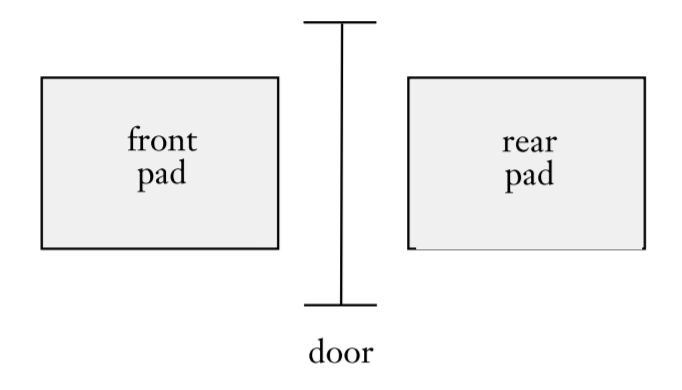
\includegraphics[scale=0.4]{assets/door.png}
\end{center}
Here:
\begin{itemize}
    \item The front pad is there is to detect the presence of a person who is about to walk through the doorway. 
    \item The rear pad is there so that the controller can hold the door open long enough for the person to pass all the way through while also ensuring that no one behind door is hit by the door. 
\end{itemize}
The controller is in either of two states: \code{OPEN} or \code{CLOSED}. This represents the condition of the door. There are also \emph{four} possible input conditions: 
\begin{itemize}
    \item \code{FRONT}: A person is standing on the pad in front of the doorway (the front pad).
    \item \code{REAR}: A person is standing on the pad to the rear of the doorway (the rear pad).
    \item \code{BOTH}: People are standing on both pads. 
    \item \code{NEITHER}: No one is standing on either pad.
\end{itemize}
The corresponding state diagram is: 
\begin{center}
    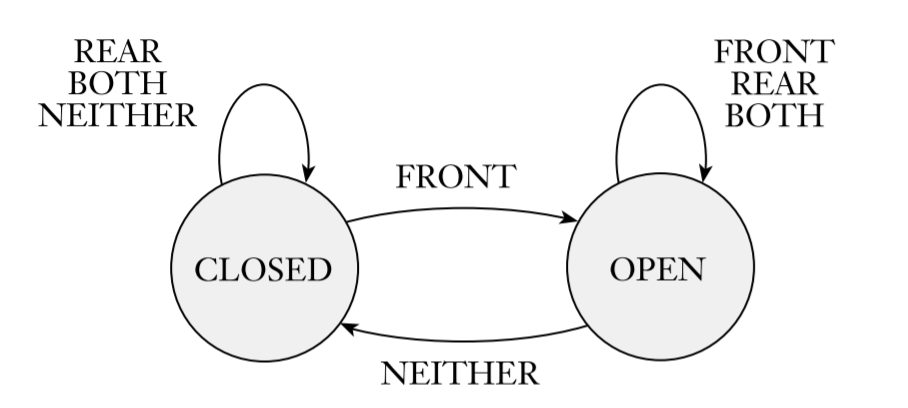
\includegraphics[scale=0.4]{assets/door_state.png}
\end{center}
And the corresponding transition table: 
\begin{center}
    \begin{tabular}{c|c c c c} 
                & \code{NEITHER} & \code{FRONT} & \code{REAR} & \code{BOTH} \\ 
            \hline
            \code{CLOSED} & \code{CLOSED} & \code{OPEN} & \code{CLOSED} & \code{CLOSED} \\ 
            \code{OPEN} & \code{CLOSED} & \code{OPEN} & \code{OPEN} & \code{OPEN} 
    \end{tabular}
\end{center}

The controller moves from state to state depending on what input it receives. For example: 
\begin{itemize}
    \item When it starts off in the \code{CLOSED} state and receives input \code{NEITHER} or \code{REAR}, it remains in the \code{CLOSED} state. In the state diagram, if we start at the \code{CLOSED} circle (state), both \code{NEITHER} and \code{REAR} loop back to \code{CLOSED}.
    \item Again, when the controller is in the \code{CLOSED} state and it receives the \code{BOTH} input, then it stays in the \code{CLOSED} state because opening the door may knock someone over on the rear pad (as the door opens towards the rear side).
    \item If the controller is in the \code{OPEN} state, then receiving the inputs \code{FRONT}, \code{REAR}, or \code{BOTH} will result in the controller remaining \code{OPEN}. However, if it receives the \code{NEITHER} input, then it goes to a \code{CLOSED} state. 
\end{itemize}
Essentially, \textbf{for the state diagram}, start at the initial state (circle) and follow the arrow depending on what input signals are received. \textbf{For the transition table}, look at the row corresponding to the initial state and the column corresponding to the input; the resulting cell will be the new state of the controller.

\bigskip

The figures used above (the state diagram and transition table) are both standard ways of representating a finite automaton. While this door may be very simple (due to the fact that it only really needs to store an extremely small amount of memory), in reality, we may be dealing with other devices with somewhat more memory. 

\bigskip

Both finite automata and their probablistic counterpart \textbf{Markov chains} are useful tools when we want to attempt to recognize patterns in data. 

\subsection{From a Mathematical Perspective}
Consider the following figure, which depicts a finite automaton called $M_1$:
\begin{center}
    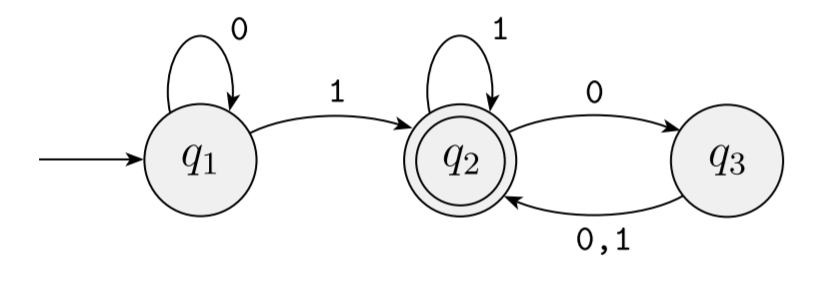
\includegraphics[scale=0.4]{assets/finite_automaton_1.png}
\end{center}
There are a few things to note here: 
\begin{itemize}
    \item The above figure for $M_1$ is called the \textbf{state diagram} of $M_1$. 
    \item $M_1$ has three \textbf{states}, labeled $q_1$, $q_2$, and $q_3$. 
    \item The \textbf{start state} is the state indicated by the arrow pointing at it from nowhere. In the case of the above state diagram, this would be $q_1$. 
    \item The \textbf{accept state} is the state with a \underline{double circle}. In the case of the above state diagram, this would be $q_2$. 
    \item The \textbf{transitions} are the arrows going from one state to another. 
\end{itemize}
For a given input string, \underline{this} automaton processes that string and produces an output that is either \code{ACCEPT} or \code{REJECT}. For this automaton, the processing works like so: 
\begin{enumerate}
    \item Here, the processing begins in $M_1$'s start state. 
    \item Then, the automaton receives the symbols from the input string one by one from left to right. 
    \item After reading each symbol, $M_1$ moves from one state to another along the transition that has that symbol as its label. 
    \item When it reads the last symbol, $M_1$ produces its output. The output is \code{ACCEPT} if $M_1$ is now in an accept state and \code{REJECT} if it is not. 
\end{enumerate}
As an example, suppose we give $M_1$ the input string \code{1101}. Then, the processing proceeds as follows: 
\begin{itemize}
    \item Start in state $q_1$. 
    \item Read \code{1}. Transition from $q_1$ to $q_2$. 
    \item Read \code{1}. Transition from $q_2$ to $q_2$. 
    \item Read \code{0}. Transition from $q_2$ to $q_3$. 
    \item Read \code{1}. Transition from $q_3$ to $q_2$. 
    \item \code{ACCEPT} because $M_1$ is in an accept state $q_2$ at the end of the input. 
\end{itemize}
So, really, what matters is that we \emph{end up} at the accept state. 

\subsection{Formal Definition of a Finite Automaton}
A finite automaton has several parts.
\begin{itemize}
    \item It has a set of states and rules for going from one state to another, depending on the input symbol.
    \item It has an input alphabet that indicates the allowed input symbols. 
    \item It has a start state and a set of accept states. 
\end{itemize}
We use something called a \textbf{transition function}, often denoted $\delta$, to define the rules for moving. If the finite automaton has an arrow from a state $x$ to a state $y$ labeled with the input symbol \code{1}, that means that if the automaton is in state $x$ when it reads a \code{1}, it then moves to state $y$. We can indicate the same thing with the transition function by saying that: 
\[\delta(x, \code{1}) = y\]
All of this leads to the formal definition:
\begin{definition}{Finite Automaton}{}
    A \textbf{finite automaton} is a 5-tuple $(Q, \Sigma, \delta, q_0, F)$ where: 
    \begin{enumerate}
        \item $Q$ is a finite set called the \textbf{states}.
        \item $\Sigma$ is a finite set called the \textbf{alphabet}.
        \item $\delta: Q \times \Sigma \mapsto Q$ is the \textbf{transition function}.
        \item $q_0 \in Q$ is the \textbf{start state}.
        \item $F \subseteq Q$ is the \textbf{set of accept states} (sometimes also called \emph{final states}).
    \end{enumerate}
\end{definition}
\textbf{Remark:} $F$ can be the empty set $\emptyset$, which means that there are 0 accept states.

\subsection{Applying the Definition}
Consider again $M_1$:
\begin{center}
    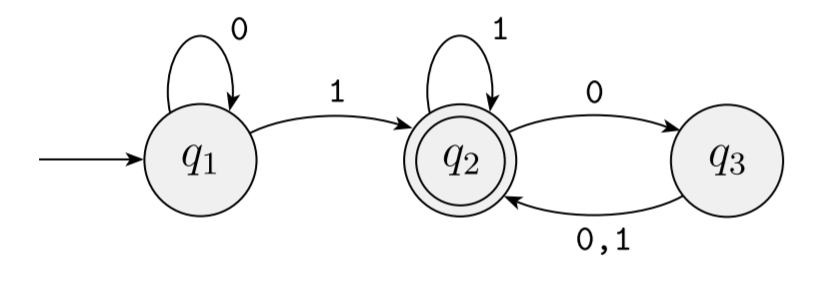
\includegraphics[scale=0.4]{assets/finite_automaton_1.png}
\end{center}
Using the formal definition above, we can describe $M_1$ formally be writing $M_1 = (Q, \Sigma, \delta, q_1, F)$, where: 
\begin{itemize}
    \item $Q = \{q_1, q_2, q_3\}$
    \item $\Sigma = \{\code{0, 1}\}$
    \item $\delta$ is defined as: 
    \begin{center}
        \begin{tabular}{c|c c}
                  & \code{0} & \code{1} \\ 
            \hline 
            $q_1$ & $q_1$    & $q_2$ \\ 
            $q_2$ & $q_3$    & $q_2$ \\ 
            $q_3$ & $q_2$    & $q_2$ 
        \end{tabular}
    \end{center}
    \item $q_1$ is the start state. 
    \item $F = \{q_2\}$. 
\end{itemize}

\subsection{Machine and Language}
If $A$ is the set of all strings (i.e. language) that machine $M$ accepts, we say that $A$ is the \textbf{language of machine} $M$, write $L(M) = A$, and say that $M$ recognizes $A$. 

\bigskip

A machine may accept \emph{several strings}, but it always recognizes \underline{one language}. A machine can accept no strings; in this case, it still recognizes the empty language $\emptyset$. 

\bigskip

If we consider our example automaton $M_1$, then define: 
\[A = \{w \mid w \text{ contains at least one \code{1} or an even number of \code{0}s follow the last \code{1}}\}\]
Which means that $L(M_1) = A$, of equivalently, $M_1$ recognizes $A$. 

\subsubsection{Example 1: Simple Finite Automaton}
Consider the following state diagram for the finite automaton $M_2$:
\begin{center}
    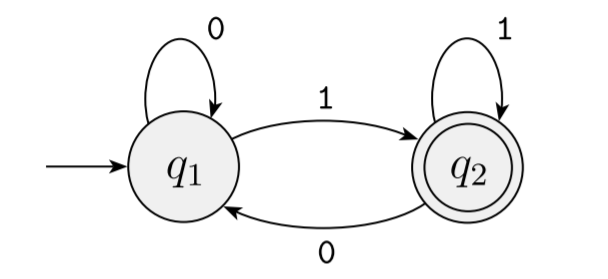
\includegraphics[scale=0.4]{assets/finite_automaton_2.png}
\end{center}
Here, the formal description of $M_2$ is as follows: 
\[M_2 = (\{q_1, q_2\}, \{\code{0, 1}\}, \delta, q_1, \{q_2\})\]
Where $\delta$ is: 
\begin{center}
    \begin{tabular}{c|c c}
            & \code{0} & \code{1} \\
        \hline  
        $q_1$ & $q_1$ & $q_2$ \\ 
        $q_2$ & $q_1$ & $q_2$
    \end{tabular}
\end{center}
To figure out what $A$ is, we try a few different strings.
\begin{center}
    \begin{tabular}{c|c}
        \textbf{String Input} & \textbf{Output} \\ 
        \hline 
        $\epsilon$ & \code{REJECT} \\ 
        \code{1} & \code{ACCEPT} \\ 
        \code{0} & \code{REJECT} \\ 
        \code{01} & \code{ACCEPT} \\ 
        \code{10} & \code{REJECT} \\ 
        \code{11} & \code{ACCEPT}
    \end{tabular}
\end{center}
It's quite clear that $A$ is simply the set of all strings that end with \code{1}. So:
\[A = \{w \mid w \text{ ends with \code{1}.}\}\]

\subsubsection{Example 2: Finite Automaton}
Consider the following state diagram for the finite automaton $M_3$:
\begin{center}
    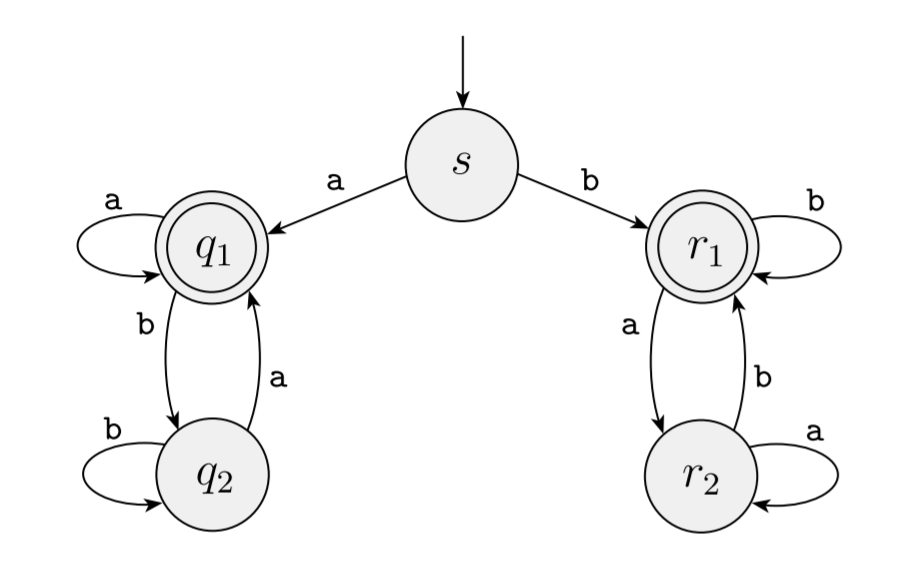
\includegraphics[scale=0.4]{assets/finite_automaton_3.png}
\end{center}
Here, the formal description of $M_3$ is as follows: 
\[M_3 = (\{s, q_1, q_2, r_1, r_2\}, \{\code{a, b}\}, \delta, s, \{q_1, r_1\})\]
Where $\delta$ is: 
\begin{center}
    \begin{tabular}{c|c c}
            & \code{a} & \code{b} \\
        \hline  
        $s$  & $q_1$ & $r_1$ \\ 
        $q_1$ & $q_1$ & $q_2$ \\ 
        $q_2$ & $q_1$ & $q_2$ \\ 
        $r_1$ & $r_2$ & $r_1$ \\ 
        $r_2$ & $r_2$ & $r_1$ \\
    \end{tabular}
\end{center}
Here, we note that we cannot end at the start state. In other words, when we start with \code{a}, we take the left branch to $q_1$. In the left branch, notice how when we end with \code{a}, we will always end up at $q_1$, the accept state. So, it follows that a string like the one below is acceptable: 
\[\code{a}w_2 w_3 \dots w_{n - 1} \code{a} \qquad w_i \in \{\code{a, b}\}\]
Likewise, if we start with \code{b}, we take the right branch to $r_1$. In the right branch, if our string ends with \code{b}, we will always end up at $r_1$. So, it follows that a string like the one below is also acceptable:
\[\code{b}w_2 w_3 \dots w_{n - 1} \code{b} \qquad w_i \in \{\code{a, b}\}\]
In other words, for this automaton, a string that starts and ends with the same symbol is accepted. That is: 
\[A = \{w \mid w \text{ starts and ends with the same symbol.}\}\]

\subsubsection{Example 3: Complicated Finite Automaton}
Sometimes, it is hard to describe a finite automaton by state diagram. In this case, we may end up using a formal description to specify the machine. Consider the following example with the alphabet: 
\[\Sigma = \{\code{RESET, 0, 1, 2}\}\]
Where \code{RESET} is treated as one symbol. For each $i \geq 1$, define $A_i$ to be the language of all strings where the sum of the numbers is a multiple of $i$, except that the sum is reset to 0 whenever the symbol \code{RESET} appears. For each $A_i$, we have a finite automaton $B_i$ which recognizes $A_i$. We define $B_i$ formally like so: 
\[B_i = (Q_i, \Sigma, \delta_i, q_0, \{q_0\})\]
Where $Q_i = \{q_0, q_1, q_2, \dots, q_{i - 1}\}$ and the transition function $\delta_i$ is defined so that for each $j$, if $B_i$ is in $q_j$ (i.e. $B_i$ is in state $q_j$), the running sum is $j$ modulo $i$. In other words, for each $q_j$ define: 
\[\delta_{i}(q_j, \code{0}) = q_j\]
\[\delta_{i}(q_j, \code{1}) = q_k \text{  where } k = j + 1 \text{ modulo } i\]
\[\delta_{i}(q_j, \code{2}) = q_k \text{  where } k = j + 2 \text{ modulo } i\]
\[\delta_{i}(q_j, \code{RESET}) = q_0\]

\bigskip

For example, suppose we have the following state machine $B_3$ which uses the same alphabet described above:
\begin{center}
    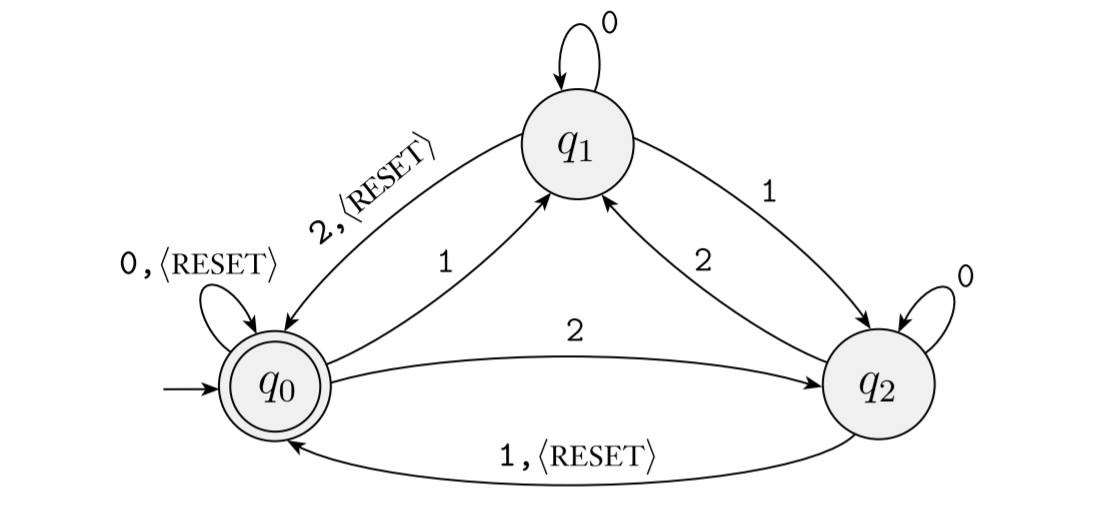
\includegraphics[scale=0.4]{assets/finite_automaton_4.png}
\end{center}
The formal description of $B_3$ is as follows: 
\[B_3 = (\{q_0, q_1, q_2\}, \{\code{RESET, 0, 1, 2}\}, \delta, q_0, \{q_0\})\]
Where $\delta$ is defined by: 
\begin{center}
    \begin{tabular}{c|c c c c}
              & \code{RESET} & \code{0} & \code{1} & \code{2} \\
        \hline  
        $q_0$ & $q_0$        & $q_0$    & $q_1$    & $q_2$    \\ 
        $q_1$ & $q_0$        & $q_1$    & $q_2$    & $q_0$    \\
        $q_2$ & $q_0$        & $q_2$    & $q_0$    & $q_1$
    \end{tabular}
\end{center}
So, as an example, let's suppose we have the string \code{01212}. The sum of these numbers is:
\[0 + 1 + 2 + 1 + 2 = 6 \implies 6 \equiv \boxed{0} \mod{3}\]
We expect the automaton to finish at the accept state as 6 is a multiple of 3. Running through the automaton, we have: 
\begin{itemize}
    \item Input: \code{0}. Start at $q_0$, end at $q_0$.
    \item Input: \code{1}. Start at $q_0$, end at $q_1$. So, our automaton is at state $q_1$.
    \item Input: \code{2}. Start at $q_1$, end at $q_0$. So, our automaton is at state $q_0$.
    \item Input: \code{1}. Start at $q_0$, end at $q_1$. So, our automaton is at state $q_1$.
    \item Input: \code{2}. Start at $q_1$, end at $q_0$. So, our automaton is at state $q_0$.
\end{itemize}
Therefore, we are at an accept state as our string \code{01212} sums up to a multiple of 3. Of course, if there are any \code{RESET}s in our string, we can disregard everything up to and including the \emph{last} \code{RESET} as \code{RESET} puts us back at the start. That is, for instance, the string \code{0121 RESET 21011 RESET 01212} will put the state machine in the same state as \code{01212}.

\bigskip

So, it follows that our state machine recognizes the set $A_3$, which consists of all strings where all digits sum up to 0 modulo 3. That is: 
\[A_3 = \left\{w \mid \sum_{\code{d} \in w} d = 0 \Mod{3}\right\}\]
\emph{Note:} If any \code{RESET}s are in the string, we can omit everything in the string \emph{up to and including} the last \code{RESET}.



\subsection{Formal Definition of Computation}
To review, let $M = (Q, \Sigma, \delta, q_0, F)$ be a finite automaton and let $w = w_1 w_2 \dots w_n$ be a string where each $w_i \in \Sigma$. Then, we say that $M$ accepts $w$ if a sequence of states $r_0, r_1, \dots, r_n$ in $Q$ exists with three conditions: 
\begin{enumerate}
    \item $r_0 = q_0$: The machine starts in the start state. 
    \item $\delta(r_i, w_{i + 1}) = r_{i + 1}$, for $i = 0, \dots, n - 1$: The machine goes from state to state according to the transition function. 
    \item $r_n \in F$: The machine accepts its input if it ends up in an accept state. 
\end{enumerate}
In particular, we say that $M$ recognizes language $A$ if $A = \{w \mid M \text{ accepts } w\}$.
\begin{definition}{Regular Language}{}
    A language is called a \textbf{regular language} if some finite automaton recognizes it.
\end{definition}

\subsubsection{Example 1: State Machine}
Recall, for example, our state machine $B_3$ in the previous lecture notes. If $w$ was the string:
\begin{verbatim}
    10 RESET 22 RESET 012
\end{verbatim}
Then, $M_5$ accepts $w$ according to the formal definition of computation because the sequence of states it enters when computing on $w$ is: 
\[q_0, q_1, q_1, q_0, q_2, q_1, q_0, q_0, q_1, q_0\]
In particular:
\begin{enumerate}
    \item The machine starts in the start state as expected. 
    \item The machine goes from state to state as expected. 
    \item The machine ends at the accept state. 
\end{enumerate}

\subsection{Designing Finite Automata}
A helpful approach when designing various types of automata is: 
\begin{mdframed}[]
    \emph{Put yourself in the place of the machine you are trying to design and then see how you would go about performing the machine's task.}
\end{mdframed} 
Suppose you are given some language and want to design a finite automaton that recognizes it. Given some input string, your goal is to determine if it is a member of the language the automaton is supposed to recognize. However, you can only see each symbol one at a time; after each symbol, you need to decide whether the string seen is in the language. The hardest part is that you need to figure out what you need to remember about the string as you are reading it. Remember: you only have a finite number of states, which means finite memory (hence, \emph{finite} automata). 

\subsubsection{Example 1: Designing a Finite Automaton}
Given $\Sigma = \{\code{0, 1}\}$, suppose we need to create a finite automaton $E_2$ that recognizes the regular language of all strings that contain \code{001} as a substring. For example, \code{001}, \code{1001}, \code{0010}, \code{111111001111101} are all in the language; however, \code{0000} and \code{11} are not.

\bigskip

Well, the first thing we can do is create the set of states that will result in an \code{ACCEPT} state. This is as simple as:
\begin{center}
    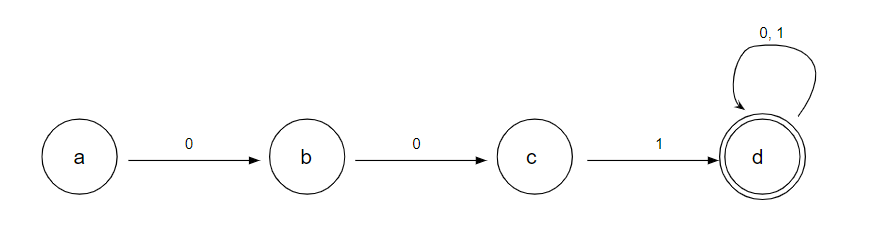
\includegraphics[scale=0.6]{assets/state_1.png}
\end{center}
Here, it's clear that a string like \code{001} will result in an \code{ACCEPT} state. Now, we need to account for any other strings. In particular, we need to account for several different possibilities:
\begin{itemize}
    \item We haven't seen any symbols associated with the pattern (e.g. we start with \code{1}s, or we saw a \code{0} and then a \code{1}). 
    \item We just saw \code{0}.
    \item We just saw \code{00}.
    \item We have seen the pattern \code{001}.
\end{itemize}
This gives us the automaton:
\begin{center}
    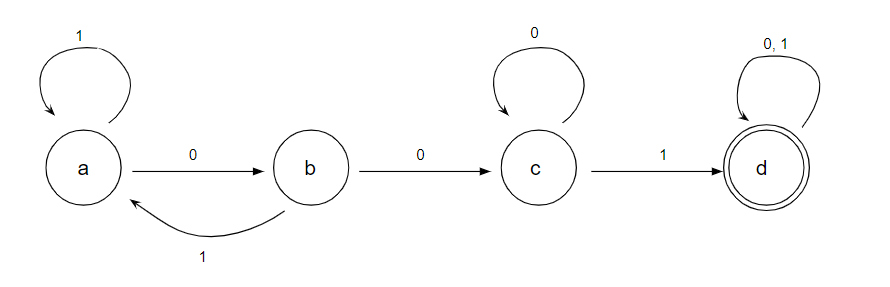
\includegraphics[scale=0.6]{assets/state_2.png}
\end{center}

\subsection{The Regular Operations}
In arithmetic, the basic objects are numbers and the tools are operations for manipulating them (e.g. $+$ or $\times$). In the theory of computation, the objects are languages and the tools include operations designed for manipulating them. We call these \textbf{regular operations}.

\begin{definition}{}{}
    Let $A$ and $B$ be languages. We define the regular operations \textbf{union}, \textbf{concatenation}, and \textbf{star} as follows: 
    \begin{itemize}
        \item \textbf{Union:} $A \cup B = \{x \mid x \in A \text{ or } x \in B\}$.
        \item \textbf{Concatenation:} $A \circ B = \{xy \mid x \in A \text{ and } y \in B\}$
        \item \textbf{Star:} $A^* = \{x_1 x_2 \dots x_k \mid k \geq 0 \text{ and each } x_i \in A\}$
    \end{itemize}
\end{definition}
\textbf{Remarks:}
\begin{itemize}
    \item The union operation simply takes all strings in both $A$ and $B$ and puts them together into one language.
    \item The concatenation operation attaches a string from $A$ in front of a string from $B$ in \emph{all possible ways to get the strings in the new language}.
    \item The star operation attaches any number of strings in $A$ together to get a string in the new language. Note that \emph{any number} includes 0, so the empty string $\epsilon$ is always in $A^*$.
\end{itemize}

\subsubsection{Example 1: String Manipulation}
Suppose $\Sigma = \{\code{a, b, ..., z}\}$ is the standard 26 letters. Define the two languages to be:
\[A = \{\code{good, bad}\}\]
\[B = \{\code{boy, girl}\}\]
Then: 
\begin{itemize}
    \item $A \cup B = \{\code{good, bad, boy, girl}\}$
    \item $A \circ B = \{\code{goodboy, goodgirl, badboy, badgirl}\}$
    \item $A^* = \{\epsilon, \code{good, bad, goodgood, goodbad, badgood, badbad, goodgoodgood, ...}\}$
\end{itemize}

\subsection{Justifying DFAs}
To prove that the DFA that we build, $M$, actually recognizes the language $L$, we ask the following questions: 
\begin{enumerate}
    \item Is every string accepted by $M$ in $L$?
    \item Is every string from $L$ accepted by $M$?\footnote{The contrapositive version is: Is every string rejected by $M$ not in $L$?}
\end{enumerate}
A string is accepted by a DFA when: 
\[ L(M) = \{ w \mid \delta^{*}(q_0, w) \in F \} \]
Where $\delta^*$ is defined by: 
\[\delta^{*}(q, w) = \begin{cases}
    q & w = \epsilon \\ 
    \delta(q, c) & w = c, c \in \Sigma \\ 
    \delta^{*}(\delta(q, c), w') & w \subset w', c \in \Sigma, w' \in \Sigma^*
\end{cases}\]


\subsection{Complementation of DFAs}
\begin{theorem}{Complementation}{}
    If $A$ is a regular language over $\{0, 1\}^*$, then so is its complement. 
\end{theorem}
\textbf{Remarks:}
\begin{itemize}
    \item This is essentially the same thing as saying that the class of regular languages is closed under complementation.
    \item How do we apply this? Let $A$ be a regular language. Then, there is a DFA $M = (Q, \Sigma, \delta, q_0, F)$ such that $L(M) = A$. We want to build a DFA $M'$ whose language is $\overline{A}$. Define: 
    \[M' = (Q, \Sigma, \delta, q_0, Q \setminus F)\]
\end{itemize}

\begin{proposition}
    $M'$ accepts $A^c$.
\end{proposition}

\begin{mdframed}[]
    \begin{proof}
        Because $M$ accepts $A$, we define $A$ to be: 
        \[A = \{w \mid M \text{ accepts } w\} = \{w \mid \delta^{*}(q_0, w) \in F\}\]
        Recall that $\delta^{*}(q, w)$ is the state reached from $q$ after reading the word $w$. Taking the complement of $A$, we have: 
        \[A^c = \{w \mid w \notin A\} = \{w \mid \delta^{*}(q_0, w) \notin F\} = \{w \mid \delta^{*}(q_0, w) \in Q \setminus F\}\]
        So, $M'$ accepts $A^c$. 
    \end{proof}
\end{mdframed}

\subsubsection{Example 1: Building DFA}
Construct a DFA that recognizes $\{w \mid w \text{ contains the substring baba}\}$.

\begin{mdframed}[nobreak=true]
    \begin{center}
        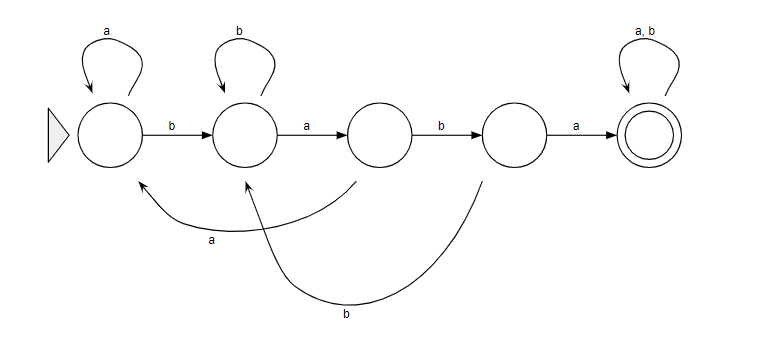
\includegraphics[scale=0.7]{assets/baba_state.png}
    \end{center}
\end{mdframed}

\subsubsection{Example 2: Building DFA}
Construct a DFA that recognizes $\{w \mid w \text{ doesn't contain the substring baba}\}$.

\begin{mdframed}[nobreak=true]
    \begin{center}
        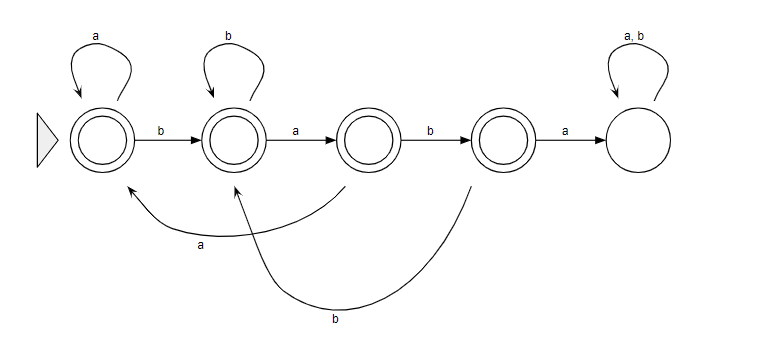
\includegraphics[scale=0.7]{assets/not_baba_state.png}
    \end{center}
\end{mdframed}

\subsection{Regular Operations}
In arithmetic, the basic objects are numbers and the tools are operations for manipulating them (e.g. $+$ or $\times$). In the theory of computation, the objects are languages and the tools include operations designed for manipulating them. We call these \textbf{regular operations}.

\begin{definition}{}{}
    Let $A$ and $B$ be languages. We define the regular operations \textbf{union}, \textbf{concatenation}, and \textbf{star} as follows: 
    \begin{itemize}
        \item \textbf{Union:} $A \cup B = \{x \mid x \in A \text{ or } x \in B\}$.
        \item \textbf{Concatenation:} $A \circ B = \{xy \mid x \in A \text{ and } y \in B\}$
        \item \textbf{(Kleene) Star:} $A^* = \{x_1 x_2 \dots x_k \mid k \geq 0 \text{ and each } x_i \in A\}$
    \end{itemize}
\end{definition}
\textbf{Remarks:}
\begin{itemize}
    \item The union operation simply takes all strings in both $A$ and $B$ and puts them together into one language.
    \item The concatenation operation attaches a string from $A$ in front of a string from $B$ in \emph{all possible ways to get the strings in the new language}.
    \item The star operation attaches any number of strings in $A$ together to get a string in the new language. Note that \emph{any number} includes 0, so the empty string $\epsilon$ is always in $A^*$.
\end{itemize}
Note that we can prove the union operation today, but we cannot prove the concatenation or star operators until later.

\subsubsection{Union}
\begin{theorem}{}{}
    The class of regular languages over a fixed alphabet $\Sigma$ is closed under the union operator. 
\end{theorem}
\textbf{Remark:} In other words, if $A_1$ and $A_2$ are regular language, so is $A_1 \cup A_2$.

\bigskip 

Essentially, we want to show that if we have two regular languages $A$ and $B$, then the union of them must also be regular. Thus, we want to show that if $M_1$ is the DFA for $A$ and $M_2$ is the DFA for $B$, then there is a DFA that recognizes $A \cup B$:
\begin{itemize}
    \item The goal is to build a DFA that recognizes $A \cup B$. 
    \item The strategy is to use DFAs that recognize each of $A$ and $B$. 
\end{itemize}
A basic sketch of this proof is as follows: 
\begin{mdframed}[]
    \begin{proof}
        We want to show that $M$ accepts $w$ if $M_1$ accepts $w$ \emph{or} $M_2$ accepts $w$. Let $A$ and $B$ be any two regular languages over $\Sigma$. Given:
        \[M_1 = (Q_1, \Sigma, \delta_1, q_1, F_1) \qquad L(M_1) = A\]
        \[M_2 = (Q_2, \Sigma, \delta_2, q_2, F_2) \qquad L(M_2) = B\]
        We want to show that $A \cup B$ is regular. The idea is to run these two DFAs $M_1$ and $M_2$ in parallel. So, we define: 
        \[M = (Q_1 \times Q_2, \Sigma, \delta, (q_1, q_2), F)\]
        Where, for $r \in Q_1$, $s \in Q_2$, and $x \in \Sigma$, we define:
        \[\delta((r, s), x) = (\delta_{1}(r, x), \delta_{2}(s, x))\]
        \[F = \{(r, s) \mid r \in F_1 \text{ or } s \in F_2\}\]
        \begin{mdframed}[]
            Note that it is not $\{(r, s) \mid r \in F_1 \text{ and } s \in F_2\}$ because this would be under intersection. Likewise, it is not $F_1 \times F_2$ because it is also intersection. 
        \end{mdframed}

        (And so on...)
    \end{proof}
\end{mdframed}

\subsubsection{Intersection}
\begin{mdframed}[]
    \begin{proof}
        The proof is left for another day.
    \end{proof}
\end{mdframed}

\begin{theorem}{}{}
    The class of regular languages is closed under the concatenation operation.
\end{theorem}
\textbf{Remark:} In other words, if $A_1$ and $A_2$ are regular language, then so is $A_1 \circ A_2$.

\bigskip 

How would you prove that the class of regular languages is closed under intersection? The idea is that:
\[A \cap B = (A^c \cup B^c)^c\]
We've already shown that the union is closed and so is its complement. 

\subsubsection{Payoff}
Consider the set: 
\[
    \{w \mid w \text{ contains neither the substrings aba nor baab}\}  
\]
Is this a regular set? 

\begin{mdframed}[]
    We know that:
    \[A = \{w \mid w \text{ contains aba as a substring}\}\]
    \[B = \{w \mid w \text{ contains baab as a substring}\}\]
    From which we know: 
    \[\overline{A} \cap \overline{B} = \overline{A \cup B}\]
\end{mdframed}










\newpage 

\section{Nondeterministic Finite Automata (1.2)}
In a deterministic finite automata, when the machine was in a given state and reads the next input symbol, we knew that the next state is; that's why it's called \emph{determinstic}, because it was already determined. \textbf{However}, in a \emph{nondeterministic} machine, several choices may exist for the next state at any point. In general, nondeterminism is a \emph{generalization} of determinism; that is, every deterministic finite automaton is automatically a nondeterminism finite automaton.

\subsection{The Differences Between DFA and NFA}
\begin{center}
    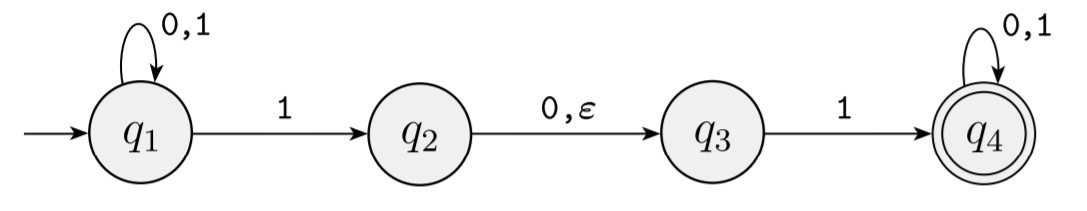
\includegraphics[scale=0.4]{assets/nfa_1.png}
    
    \textbf{Figure:} The nondeterministic finite automaton $N_1$. 
\end{center}

\begin{center}
    \begin{tabular}{p{3in}|p{3in}}
        \textbf{DFA} & \textbf{NFA} \\ 
        \hline 
        \begin{itemize}
            \item Every state of a DFA always has exactly one exiting transition arrow for each symbol in the alphabet.
            \item There is a unique computation path for each input. 
            \item Labels on the transition arrows are symbols from the alphabet. 
        \end{itemize} 

        & \begin{itemize}
            \item Not every state in an NFA needs exactly one transition arrow for each symbol. In an NFA, a state may have zero, one, or many exiting arrows for each alphabet symbol.
            \item We may allow several (or zero) alternative computations on the same input. 
            \item NFAs may have arrows labeled with members of the alphabet or $\epsilon$. Zero, one, or many arrows may exit from each state with the label $\epsilon$. For example, the above figure has one transition arrow with $\epsilon$ as a label. 
        \end{itemize}
    \end{tabular}
\end{center}

\subsection{NFA Computation}
How does an NFA compute? Suppose that we are running an NFA on an input string and come to a state with multiple ways to proceed. Suppose, in fact, that we use the NFA above: $N_1$. Additionally, suppose that we are at state $q_1$, and the next input symbol is \code{1}. 
\begin{itemize}
    \item After reading this symbol, the machine \textbf{splits into multiple copies of itself} and follows \emph{all} the possibilities in \emph{parallel}. In other words, each copy of the machine takes one of the possible ways to proceed and continues as before. 
    \item If there are subsequent choices, the machine splits again. 
    \item If the next input symbol doesn't appear on any of the arrows exiting the stae occupied by a copy of the machine, that copy of the machine dies.
    \item If any one of these copies of the machine is in an accept state at the \underline{end of the input}, the NFA \emph{accepts} the input string.
\end{itemize}
What happens when we come across a state with an $\epsilon$ symbol on an exiting arrow? Well, without reading any input, the machine splits into \emph{multiple} copies, one following each of the exiting $\epsilon$-labeled arrows and one staying at the current state. The machine, then, proceeds nondeterministically as before. So, really, $\epsilon$ transitions allow the machine to \textbf{transition between states spontaneously} without consuming any input symbols.

\begin{center}
    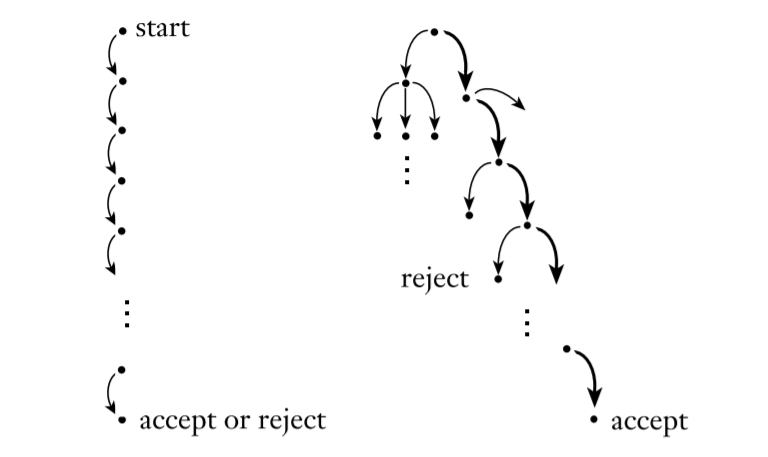
\includegraphics[scale=0.4]{assets/nfa_vs_dfa.png}

    \textbf{Figure:} Difference between deterministic computation and nondeterministic computation. 
\end{center}

We can see nondeterminism as some kind of parallel computation, where multiple independent ``threads'' or ``processes'' can be started concurrently. Whenever the NFA splits to follow several choices, that corresponds to a process ``forking'' into several children, of which each proceeds separately. Also, if one of the processes accepts, the entire computation accepts. 


\subsection{Formal Definition of NFA}
The formal definition of a nondeterministic finitne automaton is essentially the same as the one for a deterministic finitne automaton. The major difference, though, is the transition function. In particular:
\begin{center}
    \begin{tabular}{p{3in}|p{3in}}
        \textbf{DFA} & \textbf{NFA} \\ 
        \hline 
        The transition function takes a state and an input symbol, and produces the next state. & The transition function takes a state and an input symbol \emph{or} the empty string, and produces the \emph{set of possible next states}.
    \end{tabular}
\end{center}

With this in mind, we consider the definition:
\begin{definition}{Nondeterministic Finite Automaton}{}
    A \textbf{nondeterministic finite automaton} is a 5-tuple $(Q, \Sigma, \delta, q_0, F)$ where: 
    \begin{enumerate}
        \item $Q$ is a finite set called the \textbf{states}.
        \item $\Sigma$ is a finite set called the \textbf{alphabet}.
        \item $\delta: Q \times \Sigma \cup \{\epsilon\} \mapsto \PowerSet(Q)$ is the \textbf{transition function}.
        \item $q_0 \in Q$ is the \textbf{start state}.
        \item $F \subseteq Q$ is the \textbf{set of accept states} (sometimes also called \emph{final states}).
    \end{enumerate}
\end{definition}
\textbf{Remarks:}
\begin{itemize}
    \item $\Sigma \cup \{\epsilon\}$ is sometimes written as $\Sigma_{\epsilon}$.
    \item We say that $\delta(q, c)$ returns a \textbf{set} of states; more precisely, a subset of $Q$. Here, $c \in \Sigma$ or $\epsilon$ and $q \in Q$.
\end{itemize}

\subsubsection{Example: Starting NFA}
Recall the NFA $N_1$:
\begin{center}
    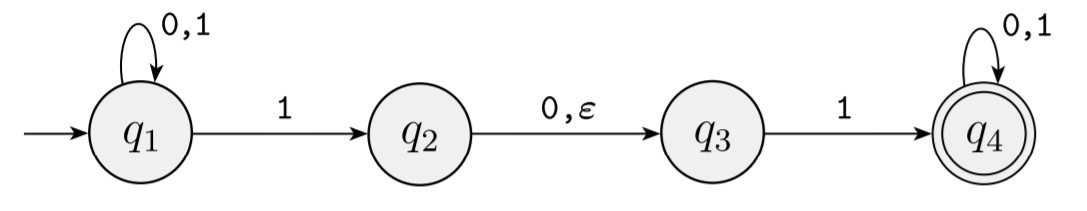
\includegraphics[scale=0.4]{assets/nfa_1.png}
\end{center}
Here, the formal description of $N_1$ is given by: 
\begin{itemize}
    \item $Q = \{q_1, q_2, q_3, q_4\}$
    \item $\Sigma = \{\code{0}, \code{1}\}$
    \item $\delta$ is given as:
    \begin{center}
        \begin{tabular}{c|c c c}
                  & \code{0} & \code{1} & $\epsilon$ \\ 
            \hline 
            $q_1$ & $\{q_1\}$ & $\{q_1, q_2\}$ & $\emptyset$ \\ 
            $q_2$ & $\{q_3\}$ & $\emptyset$ & $\{q_3\}$ \\ 
            $q_3$ & $\emptyset$ & $\{q_4\}$ & $\emptyset$ \\ 
            $q_4$ & $\{q_4\}$ & $\{q_4\}$ & $\emptyset$
        \end{tabular}
    \end{center}
    \item $q_1$ is the start state
    \item $F = \{q_4\}$
\end{itemize}

\subsection{Acceptance in an NFA}
We say that an NFA $(Q, \Sigma, \delta, q_0, F)$ accepts a string $w$ in $\Sigma^*$ if and only if we can write $w = y_1 y_2 \dots y_m$ where each $y_i \in \Sigma_{\epsilon}$ and there is a sequence of states $r_0, \dots, r_m \in Q$ such that: 
\begin{enumerate}
    \item $r_0 = q_0$. The machine starts in the start state. 
    \item $r_{i + 1} \in \delta(r_i, y_{i + 1})$ for each $i = 0, 1, \dots, m - 1$. The state $r_{i + 1}$ is one of the allowable next states when $N$ is in state $r_i$ and reading $y_{i + 1}$. Here, we note that $\delta(r_i, y_{i + 1})$ is the set of allowable next states.  
    \item $r_m \in F$. The machine accepts its input if the last state is an accept state. 
\end{enumerate}



\subsection{Equivalence of NFAs and DFAs}
Deterministic and nondeterministic finite automata both recognize the same class of languages.

\begin{theorem}{}{}
    Every nondeterministic finite automaton has an equivalent deterministic finite automaton.
\end{theorem}
\textbf{Remark:} Here, we say that two machines are equivalent if they recognize the same language. 

\bigskip 

The proof is as follows\footnote{This proof was used in our submission for HW2 Problem 3 (CSE 105, WI22). The group members involved in this submission are (only initials and the last two digits of their PID are shown): CB (67), TT (96), ASRJ (73), and me.}:
\begin{mdframed}[]
    \begin{proof}
        Let $N = (Q, \Sigma, \delta, q_0, F)$ be the NFA that recognizes the language $L$. We want to show that there is a DFA $M = (Q', \Sigma, \delta', q_0', F')$ which recognizes the same $L$. 
        \begin{enumerate}
            \item First, $Q' = \mathcal{P}(Q)$. This is because must have the states in $Q'$ to represents the possible subset of states in $Q$. In an NFA, we can make multiple copies of the automaton, which may end up at different states over time. We therefore need to account for where these copies can be in our corresponding DFA. 
 
            \item The alphabet $\Sigma$ is the same in both the NFA and DFA. 
 
            \item The transition function of the corresponding DFA is defined by: 
            \[\delta'(X, x) = \{q \in Q \mid q \in \delta(r, x) \text{ for some } r \in X \text{ or accessible via } \epsilon \text{ transitions}\}\]
            Where $X$ is a state of the DFA and $x \in \Sigma$. Because a state in an NFA can have multiple outgoing transition arrows under the same type (e.g. two outgoing arrows for \texttt{a}), we need to account for this in the corresponding NFA. This is our first condition in our $\delta'$ function; in this sense, if we consider the possible states that we can go to in the NFA, then the corresponding state in our DFA is the union of all of those possible states. 
            We must also consider that, for a given state in an NFA, there may be $\epsilon$ transitions. In case there are $\epsilon$ transitions, we need to consider where the $\epsilon$ transitions put a copy of the machine.

            \item The start state in the corresponding DFA is the set $q_0' = \{q_0\} \cup \delta^{*} (q_0, \epsilon)$. First, we note that the start state in the NFA is $q_0$; thus, the start state in the corresponding DFA must be \emph{at least} $\{q_0\}$. However, if there are any $\epsilon$ transitions from the start state, we must consider those as well since transitioning to another state from the state state via the $\epsilon$ transition doesn't consume any input. 

            \item The set of final states in the corresponding DFA is simply:
            \[F' = \{X \mid X \subseteq Q \text{ and } X \cap F \neq \emptyset\}\]
            Here, we're saying that if there are any sets in $Q'$ which contain a final state in $F$, then said set must be a final set. This is because, in a NFA, we may have multiple copies of the machine running, and if one copy stops at a final state, then the NFA is accepted (despite the other copies not necessarily being at a final state).
        \end{enumerate}
        The rest of the proof is omitted for now. 
    \end{proof}
\end{mdframed}

\subsubsection{Example: NFA to DFA}
Consider the following NFA $N$:
\begin{center}
    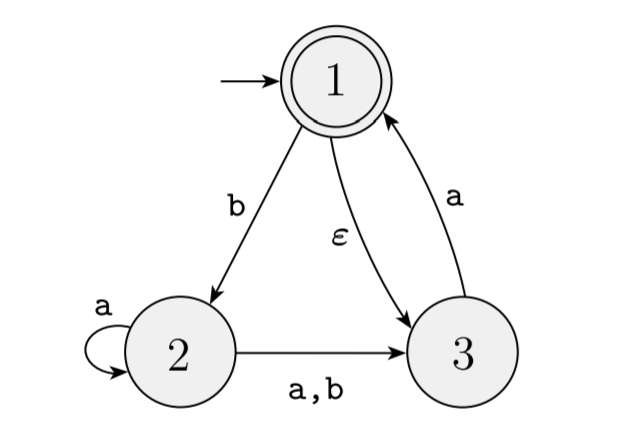
\includegraphics[scale=0.5]{assets/nfa_to_dfa_1.png}

    \textbf{Figure:} The NFA $N$. 
\end{center}
We can define $N = (Q, \Sigma, \delta, q_0, F)$ like so: 
\begin{itemize}
    \item $Q = \{\code{1}, \code{2}, \code{3}\}$
    \item $\Sigma = \{\code{a}, \code{b}\}$
    \item $\delta$ is defined by 
    \begin{center}
        \begin{tabular}{c|c c c}
                & \code{a} & \code{b} & $\epsilon$ \\ 
            \hline 
            1   & $\emptyset$ & $\{2\}$ & $\{3\}$ \\ 
            2   & $\{2, 3\}$ & $\{3\}$ & $\emptyset$ \\ 
            3   & $\{1\}$ & $\emptyset$ & $\emptyset$
        \end{tabular}
    \end{center}
    \item $q_0 = 1$
    \item $F = \{1\}$
\end{itemize}
We're now being asked to construct a corresponding DFA: 
\[D = (Q', \Sigma', \delta', q_0', F')\]
Here, it's trivial to note that: 
\begin{itemize}
    \item $Q' = \PowerSet(Q) = \{\emptyset, \{1\}, \{2\}, \{3\}, \{1, 2\}, \{1, 3\}, \{2, 3\}, \{1, 2, 3\}\}$. 
    \item $\Sigma = \{\code{a}, \code{b}\}$
    \item $q_0 = \{1, 3\}$. This is because we can start at both state 1 and 3 since 3 has an $\epsilon$ transition.
    \item $F' = \{\{1\}, \{1, 2\}, \{1, 3\}, \{1, 2, 3\}\}$. This is because we want all subsets that contain $N$'s accept state. 
\end{itemize}
The hard part is actually ``wiring'' the DFA up, i.e. the transition function. To do this, we need to analyze how the NFA acts and ``translate'' it to what the DFA would do. So, let's consider each element in $Q'$ and see how it would relate to the NFA. 
\begin{itemize}
    \item Consider $\{1\} \in Q'$. In the NFA:
    \begin{itemize}
        \item $1$ doesn't go anywhere when \code{a} is given by itself. \textbf{However}, $1$ can go to $3$ since this is an $\epsilon$ transition, and $3$ goes to $1$ when consuming \code{a}, so it follows that $\boxed{\{1\} \xrightarrow{\code{a}} \{1, 3\}}$ in the corresponding DFA. 
        \item $1$ goes to $2$ when \code{b} is given, so it follows that $\boxed{\{1\} \xrightarrow[]{\code{b}} \{2\}}$ in the corresponding DFA. 
    \end{itemize}
    \item Consider $\{2\} \in Q'$. In the NFA: 
    \begin{itemize}
        \item $2$ goes to $2$ \emph{and} $3$ when \code{a} is given, so it follows that $\boxed{\{2\} \xrightarrow{\code{a}} \{2, 3\}}$ in the corresponding DFA. 
        \item $2$ goes to $3$ when \code{b} is given, so it follows that $\boxed{\{2\} \xrightarrow[]{\code{b}} \{3\}}$ in the corresponding DFA. 
    \end{itemize}
    \item Consider $\{3\} \in Q'$. In the NFA: 
    \begin{itemize}
        \item $3$ goes to $1$ when \code{a} is given, but then it can also go to $3$ since there is an $\epsilon$ transition, so it follows that $\boxed{\{3\} \xrightarrow{\code{a}} \{1, 3\}}$. 
        \item $3$ doesn't go anywhere when \code{b} is given, so it follows that $\boxed{\{3\} \xrightarrow{\code{b}} \emptyset}$.
    \end{itemize}
\end{itemize}
We can use the above to build cases for the remaining elements in $Q'$.
\begin{itemize}
    \item Consider $\{1, 2\} \in Q'$. In the corresponding NFA, this means that there's a copy at state $1$ and a copy at state $2$. So: 
    \begin{itemize}
        \item Suppose \code{a} is given. Then, from our previous work, we know that $\{1\} \xrightarrow{\code{a}} \{1, 3\}$, and $\{2\} \xrightarrow{\code{a}} \{2, 3\}$.
        Therefore, $\boxed{\{1, 2\} \xrightarrow{\code{a}} \{1, 2, 3\}}$ (recall that we take the union).
        \item Suppose \code{b} is given. Then, we know that $\{1\} \xrightarrow{\code{b}} \{2\}$, and $\{2\} \xrightarrow[]{\code{b}} \{3\}$. Therefore, $\boxed{\{1, 2\} \xrightarrow[]{\code{b}} \{2, 3\}}$. 
    \end{itemize}
    
    \item Consider $\{1, 3\} \in Q'$. In the corresponding NFA, this means that there's a copy at state $1$ and a copy at state $3$. So: 
    \begin{itemize}
        \item Suppose \code{a} is given. Then, from our previous work, we know that $\{1\} \xrightarrow{\code{a}} \{1, 3\}$, and $\{3\} \xrightarrow{\code{a}} \{1, 3\}$.
        Therefore, $\boxed{\{1, 3\} \xrightarrow{\code{a}} \{1, 3\}}$.
        \item Suppose \code{b} is given. Then, we know that $\{1\} \xrightarrow{\code{b}} \{2\}$, and $\{3\} \xrightarrow[]{\code{b}} \emptyset$. Therefore, $\boxed{\{1, 3\} \xrightarrow[]{\code{b}} \{2\}}$. 
    \end{itemize}
    
    \item Consider $\{2, 3\} \in Q'$. In the corresponding NFA, this means that there's a copy at state $2$ and a copy at state $3$. So: 
    \begin{itemize}
        \item Suppose \code{a} is given. Then, from our previous work, we know that $\{2\} \xrightarrow{\code{a}} \{2, 3\}$, and $\{3\} \xrightarrow{\code{a}} \{1, 3\}$.
        Therefore, $\boxed{\{2, 3\} \xrightarrow{\code{a}} \{1, 2, 3\}}$.
        \item Suppose \code{b} is given. Then, we know that $\{2\} \xrightarrow{\code{b}} \{3\}$, and $\{3\} \xrightarrow[]{\code{b}} \emptyset$. Therefore, $\boxed{\{2, 3\} \xrightarrow[]{\code{b}} \{3\}}$. 
    \end{itemize}

    \item Consider $\{1, 2, 3\} \in Q'$. In the corresponding NFA, this means that there's a copy at state $1$, $2$, and $3$. So: 
    \begin{itemize}
        \item Suppose \code{a} is given. From our previous work, we know that $\boxed{\{1, 2, 3\} \xrightarrow{\code{a}} \{1, 2, 3\}}$.
        \item Suppose \code{b} is given. From our previous work, we know that $\boxed{\{1, 2, 3\} \xrightarrow{\code{b}} \{2, 3\}}$.
    \end{itemize}
\end{itemize}

This gives us the following DFA: 
\begin{center}
    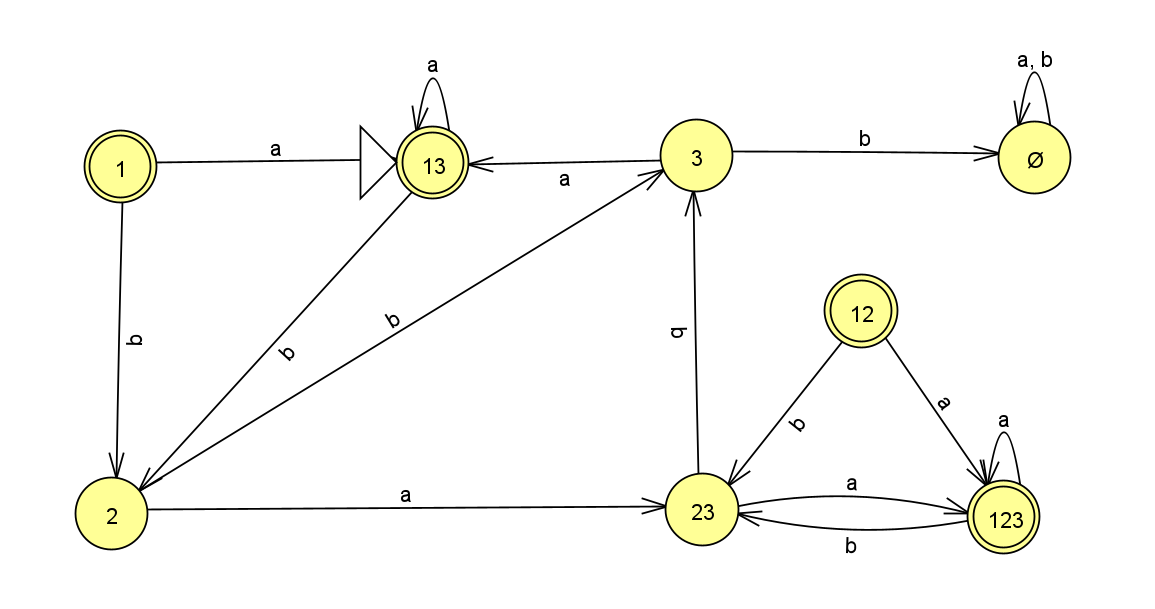
\includegraphics[scale=0.50]{assets/nfa_to_dfa_2.png}
\end{center}

However, we note a few things.
\begin{itemize}
    \item State $1$ doesn't have anything coming into it. Therefore, we can remove it.
    \item State $12$ doesn't have anything coming into it. Therefore, we can remove it.
\end{itemize}
This gives us the simplified DFA: 
\begin{center}
    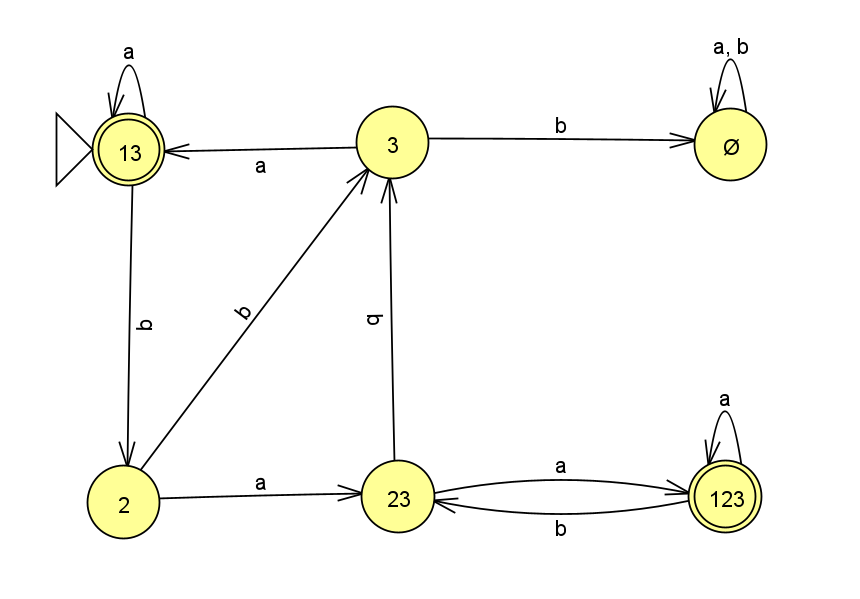
\includegraphics[scale=0.50]{assets/nfa_to_dfa_3.png}
\end{center}

\subsection{Applications of Theorem}
There are several applications of this theorem. 

\begin{corollary}{}{}
    A language is regular if and only if some nondeterministic finite automaton recognizes it.
\end{corollary}


\begin{theorem}{}{}
    The class of regular languages is closed under the union operation.
\end{theorem}

\begin{mdframed}[]
    \begin{proof}
        (Sketch.) Suppose $A_1$ and $A_2$ are regular languages. We want to show that $A_1 \cup A_2$ is regular. We can take two NFAs, $N_1$ for $A_1$ and $N_2$ for $A_2$, and combine them to make one new NFA $N$. The idea is that $N$ must accept its input if either $N_1$ and $N_2$ accepts. So, essentially, we want to run both $N_1$ and $N_2$ in parallel. To simulate this behavior, we can create a new start state $q_0$ with two $\epsilon$ transitions pointing to the original start states of $N_1$ and $N_2$ (everything else about $N_1$ and $N_2$ are left unchanged).    
    \end{proof}
\end{mdframed}

\begin{center}
    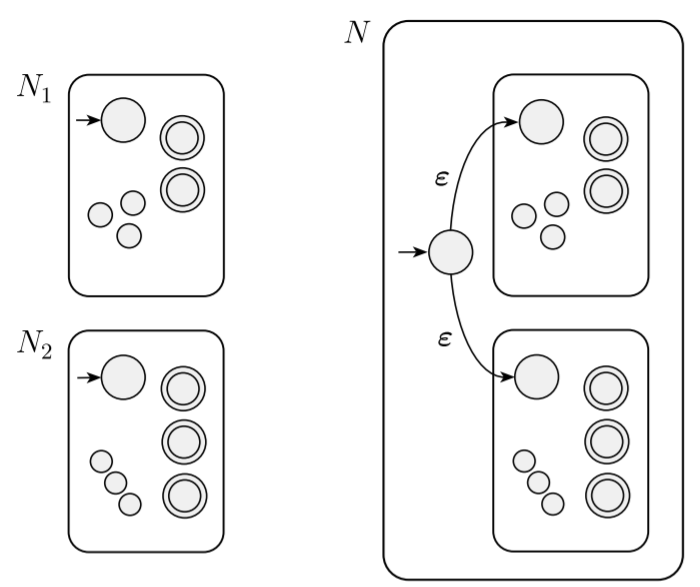
\includegraphics[scale=0.5]{assets/union_nfa.png}
\end{center}


\begin{theorem}{}{}
    The class of regular languages is closed under the concatenation operation.
\end{theorem}

\begin{mdframed}[]
    \begin{proof}
        (Sketch.) Suppose $A_1$ and $A_2$ are regular languages. We want to show that $A_1 \circ A_2$ is regular. We can take two NFAs, $N_1$ for $A_1$ and $N_2$ for $A_2$, and combine them to make one new NFA $N$. The idea for $N$ is as follows: 
        \begin{itemize}
            \item Start at the starting state for $N_1$ and remove the starting state for $N_2$. 
            \item Connect each accept state in $N_1$ to the original start state in $N_2$. The accept states in $N_1$ will no longer be accept states.  
        \end{itemize}
        By starting at the $N_1$ part of $N$, we guarantee that we will recognize some language $A_1$. Then, once we hit the original accept state in $N_1$, we can evaluate the rest of the string in $N_2$. If we hit an accept state in $N_2$, then we have recognized $A_1 \circ A_2$. 
    \end{proof}    
\end{mdframed}

\begin{center}
    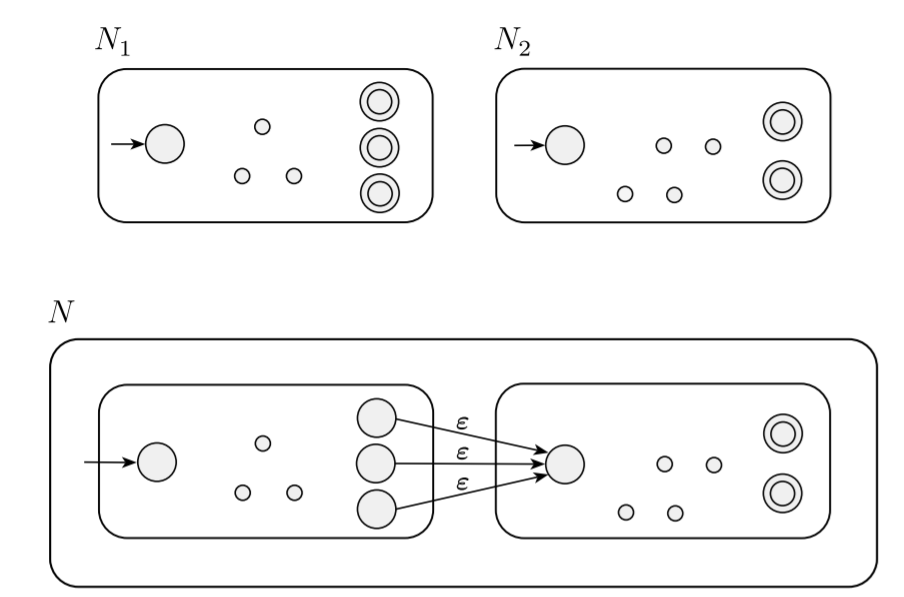
\includegraphics[scale=0.5]{assets/concat_nfa.png}
\end{center}


\begin{theorem}{}{}
    The class of regular languages is closed under the star operation.
\end{theorem}

\begin{mdframed}[]
    \begin{proof}
        (Sketch.) Suppose $A_1$ is a regular language. We want to show that $A_1^*$ is also regular. Consider the NFA $N_1$ for $A_1$. We want to modify $N_1$ so it recognizes $A_1^*$. Thus, our idea for the new NFA $N$ is as follows: 
        \begin{itemize}
            \item Because $\epsilon$ (the empty string) is valid under $A_1^*$, we must make a new start state that goes to the original start state; then, we can make the transition from the new start state to the original start state $\epsilon$. 
            \item We can connect the accept states in $N_1$ back to the original start state (not the new start state) with the labels being $\epsilon$.
            \item The accept states in $N_1$ is the same for $N$. 
        \end{itemize}
        By starting at the new start state, we can guarantee that $\epsilon$ will be accepted if it is the only thing to be read. Processing the string is as expected. However, once we reach the accept state, we need to \emph{go back} to the original start state to process the next ``word.'' This process keeps going until we no longer have any words to process. In this case, if we end off at any accept state with nothing left to read, then we accept. 
    \end{proof}
\end{mdframed}

\begin{center}
    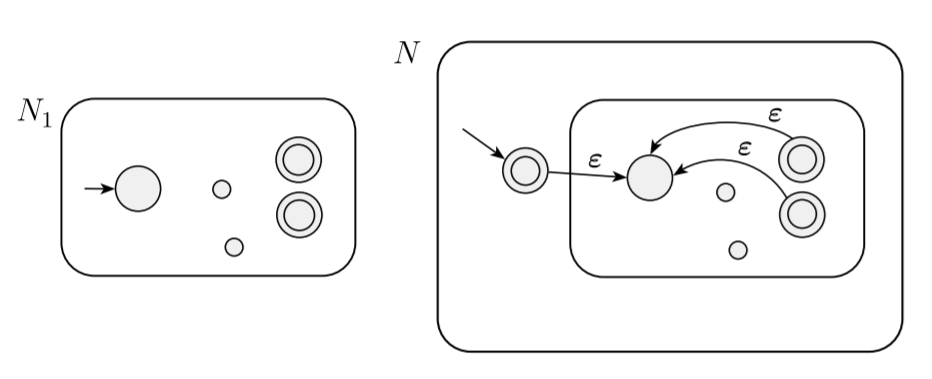
\includegraphics[scale=0.5]{assets/star_nfa.png}
\end{center}





























\newpage 
\section{Regular Expressions (1.3)}
We can use \textbf{regular expressions} (RegExp) to describe a language. An example of a regular expression is: 
\[(\code{0} \cup \code{1}) \code{0}^*\]
To give a comparison, consider the arithmetic expression:
\[(5 + 4) \times 2\]
In an arithmetic expression, the value is a number; in our case above, we would get 18. In a regular expression, the value is a \textbf{language}; in our case above, we can break the expression into multiple parts: 
\begin{itemize}
    \item $\code{0} \cup \code{1}$: This is the same thing as saying $\{\code{0}\} \cup \{\code{1}\}$, so this segment is saying that its language is $\{\code{0}, \code{1}\}$.
    \item $\code{0}^*$: This is the same thing as saying $\{\code{0}\}^*$, so its value is the language consisting of all strings containing any numbers of \code{0}s.
\end{itemize}
Putting it together, this regular expression recognizes any string which starts with \code{0} or \code{1} and ends with some number of \code{0}s. Just like how the multiplication sign $\times$ is often implicitly written (that is, we can write $2(5 + 4)$ instead of $2 \times (5 + 4)$), the concatenation sign $\circ$ is also implicitly written. That is, $(\code{0} \cup \code{1}) \code{0}^*$ is the shorthand for $(\code{0} \cup \code{1}) \circ \code{0}^*$. 

\subsection{Formal Definition of a Regular Expression}
\begin{definition}{Regular Expression}{}
    We say that $R$ is a \textbf{regular expression} if $R$ is: 
    \begin{enumerate}
        \item $a$ for some $a$ in the alphabet $\Sigma$,
        \item $\epsilon$,
        \item $\emptyset$,
        \item $(R_1 \cup R_2)$, where $R_1$ and $R_2$ are regular expressions,
        \item $(R_1 \circ R_2)$, where $R_1$ and $R_2$ are regular expressions,
        \item $(R_1^*)$, where $R_1$ is a regular expressions,
    \end{enumerate}
    In items 1 and 2, the regular expressions $a$ and $\epsilon$ represent the languages $\{a\}$ and $\{\epsilon\}$, respectively. In item 3, the regular expression $\emptyset$ represents the empty language. In items 4, 5, and 6, the expressions represent the languages obtained by taking the union or concatenation of the languages $R_1$ and $R_2$, or the star of the language $R_1$, respectively. 
\end{definition}
\textbf{Remarks:}
\begin{itemize}
    \item Remember, $\epsilon$ and $\emptyset$ are not the same. $\epsilon$ is the same thing as $\{\epsilon\}$, i.e. the language containing only the empty string; however, $\emptyset$ represents the language that doesn't contain anything. 
    \item In regular expressions, there is the notion of operator precedence. In our case, the star operation is done first, followed by concatenation, and finally union \emph{unless} parentheses change the usual order.
    \item We may omit the $\circ$ notation for concatenation. For example, $R_1 R_2$ is the same thing as $R_1 \circ R_2$.  
\end{itemize}
Additionally, we define some more notation.
\begin{itemize}
    \item Let $R^+$ be shorthand for $RR^*$. In other words, while $R^*$ has all strings that are 0 or more concatenations of strings from $R$, the language $R^+$ has all strings that are \textbf{1} or more concatenations of strings from $R$. So, really, $R^+ \cup \epsilon = R^*$. 
    \item We let $R^k$ be shorthand for the concatenation of $k$ $R$'s with each other. 
\end{itemize}
Finally, when we want to distinguish between a regular language $R$ and the language it described, we write $L(R)$ to be the language of $R$. 

\subsubsection{Example: Regular Languages}
Suppose $\epsilon = \{\code{0}, \code{1}\}$. Then, some examples of regular expressions are: 
\begin{center}
    \begin{tabular}{p{1.2in}|p{1.8in}|p{3in}}
        \textbf{RegExp} & \textbf{Examples} & \textbf{Formal Description} \\ 
        \hline 
        $\code{0}^* \code{10}^*$ & \code{1}, \code{01}, \code{0100} & $\{w \mid w \text{ contains a single } \code{1}\}$ \\ 
        \hline 
        $\Sigma^{*}\code{1}\Sigma^{*}$ & \code{1}, \code{00101101} & $\{w \mid w \text{ has at least one } \code{1}\}$ \\ 
        \hline 
        $\Sigma^{*}\code{001}\code{*}$ & \code{001}, \code{0100101} & $\{w \mid w \text{ contains the string } \code{001} \text{ as a substring}\}$ \\ 
        \hline 
        $\code{1}^* (\code{01}^+)^*$ & \code{1010110111}, \code{1110101} & $\{w \mid \text{every } \code{0} \text{ in } w \text{ is followed by at least one } \code{1}\}$ \\ 
        \hline 
        $\underbrace{(\Sigma\Sigma \dots \Sigma\Sigma)^{*}}_{n \text{ times}}$ & & $\{w \mid \text{the length of } w \text{ is a multiple of } n\}$ \\ 
        \hline 
        $\code{01} \cup \code{10}$ & \code{10}, \code{01} & $\{\code{01}, \code{10}\}$ \\ 
        \hline 
        $\code{0}\Sigma^* \code{0} \cup \code{1} \Sigma^* \code{1} \cup \code{0} \cup \code{1}$ & \code{00}, \code{11}, \code{10101}, \code{0}, \code{1} & $\{w \mid w \text{ starts and ends with the same symbol}\}$ \\ 
        \hline 
        $(\code{0} \cup \epsilon)\code{1}^*$ & \code{11111}, \code{01}, \code{0111} & $\code{01}^* \cup 1^*$ \\ 
        \hline 
        $(\code{0} \cup \epsilon)(\code{1} \cup \epsilon)$ & \code{01}, \code{1}, \code{0}, $\epsilon$ & $\{\epsilon, \code{0}, \code{1}, \code{01}\}$ \\ 
        \hline 
        $\code{1}^* \emptyset$ & & $\emptyset$ \\ 
        \hline 
        $\emptyset^*$ & $\epsilon$ & $\{\epsilon\}$
    \end{tabular}
\end{center}
\textbf{Remarks:}
\begin{itemize}
    \item Concatenating the empty set to any set yields the empty set. 
    \item The star operation on the empty set produces the set containing only the empty string. 
\end{itemize}

\subsection{Identities}
Let $R$ be any regular expression. The following identities hold:
\begin{enumerate}
    \item $R \cup \emptyset = R$. Adding the empty language to any other language will not change it. 
    \item $R \circ \epsilon = R$. Joining the empty string to any string will not change it. 
\end{enumerate}
As a warning, the following do not necessarily hold: 
\begin{enumerate}
    \item $R \cup \epsilon = R$. If $R = \code{0}$, then $L(R) = \{\code{0}\}$ but $L(R \cup \epsilon) = \{\code{0}, \epsilon\}$
    \item $R \circ \emptyset = R$. If $R = \code{0}$, then $L(R) = \{\code{0}\}$ but $L(R \circ \emptyset) = \emptyset$. 
\end{enumerate}

\subsection{Practical Applications of RegExp}
Regular expressions have practical applications. One example is in the world of compilers for programming languages. In particular, elemental objects in a programming language, called \textbf{tokens}, such as variable names and constants, can be described with regular expression. Consider the following regular expression:
\[(\code{+} \cup \code{-} \cup \epsilon)(D^+ \cup D^+ \code{.} D^* \cup D^* \code{.} D^+)\]
Where $D = \{\code{0}, \code{1}, \code{2}, \dots, \code{8}, \code{9}\}$. This regular expression describes a numerical constant which may include a fractional part and/or a sign. For example, the following strings are valid: 
\begin{itemize}
    \item \code{3.1415926}
    \item \code{+2.}
    \item \code{-.15}
\end{itemize}
After we can describe the syntax of a programming language with a regular expression in terms of its tokens, we can generate a \textbf{lexical analyzer} which processes it. 

\subsection{Generalized Nondeterministic Finite Automaton}
We now introduce a new type of finite automaton called a \textbf{generalized nondeterministic finite automaton}, also known as a GNFA. First, we briefly introduce what a GNFA is:
\begin{itemize}
    \item GNFAs are simply nondeterministic finite automata wherein the transition arrows may have any \emph{regular expressions} as labels, instead of only members of the alphabet or $\epsilon$. 
    \item The GNFA reads \emph{blocks of symbols} form the input, not necessarily just one symbol at a time.
    \item The GNFA moves along a transition arrow connecting two states by reading a block of symbols from the input, which themselves constittue a string described by the regular expression on that arrow. 
    \item GNFAs are nondeterministic, so there may be several different ways to process the same input string.
\end{itemize}
\begin{center}
    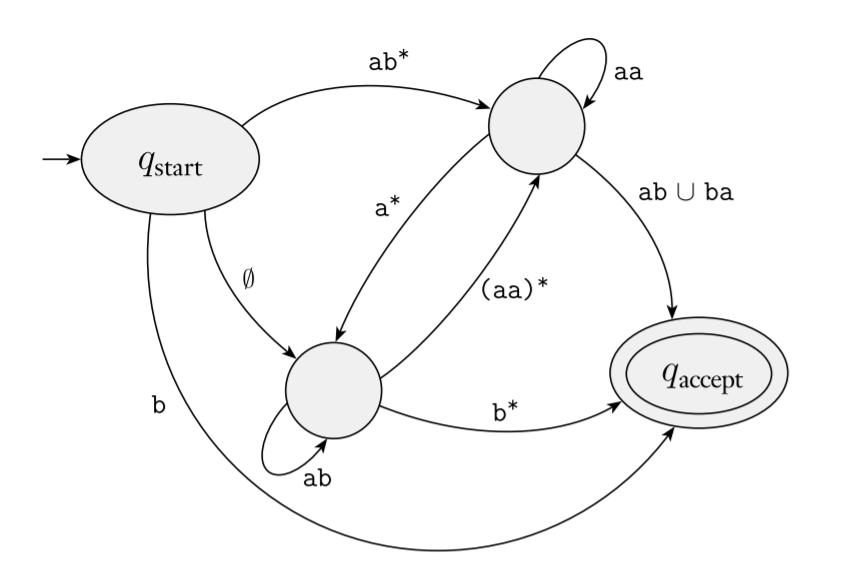
\includegraphics[scale=0.4]{assets/gnfa_ex_1.png}

    \textbf{Figure:} A generalized nondeterministic finite automaton.
\end{center}
We always require GNFAs to have a special form that meets the following conditions: 
\begin{enumerate}
    \item The \underline{start state} has transition arrows going to every other state but no arrows coming in from any other state. 
    \item There is only a single accept state, and it has arrows coming in from every other state but no arrows going to any other state. Additionally, the start state cannot be the accept state. 
    \item For all other states except the start/accept states, one arrow goes from every state to every other state and also from each state to itself. 
\end{enumerate}

\subsubsection{DFA to GNFA}
To convert a DFA to a GNFA, we do the following: 
\begin{itemize}
    \item We can add a new start state with a $\epsilon$ arrow to the old start state and a new accept state with $\epsilon$ from the old accept states. 
    \item If any arrows have multiple labels, or if there are multiple arrows going between the same two states in the same direction, replace each with a single arrow whose label is the union of the previous labels.
    \item Finally, add arrows labeled $\emptyset$ between states that have no arrows. 
\end{itemize}

\subsubsection{GNFA to Regular Expression}
We now need to convert a GNFA to a regular expression. Say that a GNFA has $k$ states. Then, because a GNFA must have a start and an accept state and they must be different from each other, we know that $k \geq 2$. If $k > 2$, we construct an equivalent GNFA with $k - 1$ states. We continue to do this until the GNFA is reduced to two states. If $k = 2$, then the GNFA has a single arrow that goes from the start state to the accept state. The label of this arrow would then be the \emph{equivalent regular expression}.

\bigskip 

The most important step in this process is constructing an equivalent GNFA with one fewer state when $k > 2$. How can we do this? Well: 
\begin{itemize}
    \item Select a state that isn't the start or accept state, rip that state out of the machine, and then repairing what is left of the machine so the same language is still recognized. Call this state $q_{\text{rip}}$.
    \item After removing $q_{\text{rip}}$, we need to repair the machine by altering the regular expressions that label each of the remaining arrows. We use these new labels because they add back the lost computations (from ripping $q_{\text{rip}}$). 
\end{itemize}
Consider the following GNFA: 
\begin{center}
    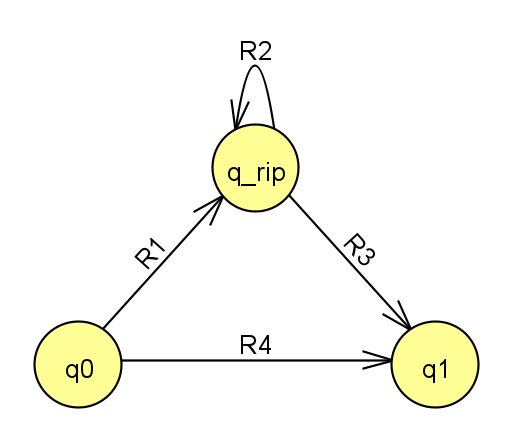
\includegraphics[scale=0.4]{assets/gnfa_before.png}
\end{center}
If we remove $q_{\text{rip}}$, we get the following GNFA: 
\begin{center}
    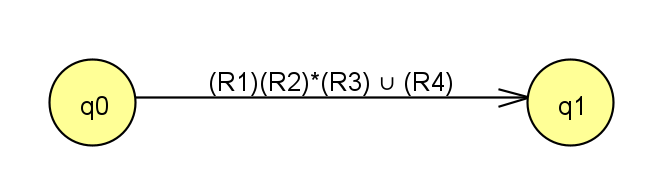
\includegraphics[scale=0.4]{assets/gnfa_after.png}
\end{center}
Essentially, in the old machine, if: 
\begin{enumerate}
    \item $q_0$ goes to $q_{\text{rip}}$ with an arrow labeled $R_1$, and 
    \item $q_{\text{rip}}$ goes to itself with an arrow labeled $R_2$, and 
    \item $q_{\text{rip}}$ goes to $q_1$ with an arrow labeld $R_3$, and 
    \item $q_0$ goes to $q_1$ with an arrow labeled $R_4$
\end{enumerate}
Then, in the new revised machine, the arrow from $q_0$ to $q_1$ gets the label 
\[(R_1)(R_2)^* (R_3) \cup (R_4)\]
We can make this change for each arrow going from any state $q_0$ to any state $q_1$, including when $q_0 = q_1$. 

\subsubsection{Formal Definition}
The formal definition of a GNFA is: 
\begin{definition}{Generalized Nondeterministic Finite Automaton}{}
    A \textbf{generalized nondeterministic finite automaton} is a 5-tuple $(Q, \Sigma, \delta, q_{\text{start}}, q_{\text{accept}})$ where 
    \begin{enumerate}
        \item $Q$ is the finite set of tuples. 
        \item $\Sigma$ is the input alphabet. 
        \item $\delta: (Q \setminus \{q_{\text{accept}}\}) \times (Q \setminus \{q_{\text{start}}\}) \mapsto \mathcal{R}$ is the transition function. 
        \item $q_{\text{start}}$ is the start state. 
        \item $q_{\text{accept}}$ is the accept state. 
    \end{enumerate}
\end{definition}
\textbf{Remarks:}
\begin{itemize}
    \item Here, $\mathcal{R}$ is the collection of all regular expressions over the alphabet $\Sigma$. 
    \item If $\delta(q_i, q_j) = R$, then the arrow from state $q_i$ to state $q_j$ has the regular expression $R$ as its label. 
\end{itemize}

\subsubsection{Convert Algorithm}
Suppose $G$ is an GNFA. Then, the $\code{CONVERT}(G)$ algorithm takes a GNFA and returns an equivalent regular expression. The algorithm works like so (Page 73): 
\begin{mdframed}[]
    $\code{CONVERT}(G)$
    \begin{enumerate}
        \item Let $k$ be the number of states of $G$. 
        \item If $k = 2$, then $G$ must consist of a start state, an accept state, and a single arrow connecting them and labeled with a regular expression $R$. So, return $R$. 
        \item Otherwise, $k > 2$ so we select any state $q_{\text{rip}} \in Q$ different from $q_{\text{start}}$ and $q_{\text{accept}}$. Let $G'$ be the GNFA $(Q', \Sigma, \delta', q_{\text{start}}, q_{\text{accept}})$ where $Q' = Q \setminus \{q_{\text{rip}}\}$ and, for any $q_i \in G' \setminus \{q_{\text{accept}}\}$ and $q_j \in Q' \setminus \{q_{\text{start}}\}$, let
        \[\delta'(q_i, q_j) = (R_1)(R_2)^* (R_3) \cup (R_4)\]
        Where $R_1 = \delta(q_i, q_{\text{rip}})$, $R_2 = \delta(q_{\text{rip}}, q_{\text{rip}})$, $R_3 = (q_{\text{rip}}, q_j)$, and $R_4 = \delta(q_i, q_j)$. 
        \item Compute $\code{CONVERT}(G')$. 
    \end{enumerate}
\end{mdframed}

\subsubsection{Example 1: DFA to Regular Expression}
Suppose we wanted to convert the following DFA to a regular expression:
\begin{center}
    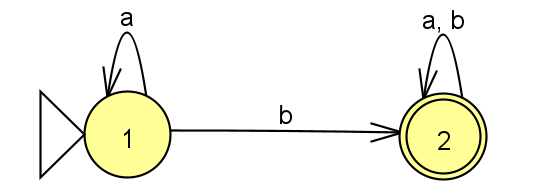
\includegraphics[scale=0.5]{assets/dfa_regex_1.png}
\end{center}

\begin{enumerate}
    \item First, we need to convert this DFA to a GNFA. This would look like: 
    \begin{center}
        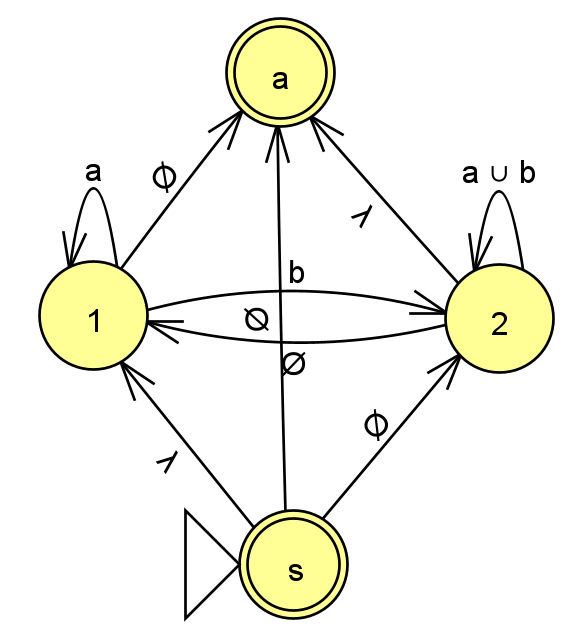
\includegraphics[scale=0.4]{assets/dfa_regex_2.png}
    \end{center}
    Here, we've made a few changes. 
    \begin{itemize}
        \item First, we added two new states: $s$ for the new \emph{start} state and $a$ for the new \emph{accept} state. We have an arrow from $s$ to $1$ (the old start state) with $\epsilon$ as its label\footnote{The software used to create these state machines use $\lambda$ instead of $\epsilon$.}. We also have an arrow from $2$ (the old accept state) to $a$ with $\epsilon$ as its label. 
        \item Next, note that there was an arrow labeled $a, b$ at state $2$. We take the \emph{union} of these two labels to get $a \cup b$. Thus, state $2$ now has an arrow with $a \cup b$ instead of $a, b$. This is because the DFA's label represents two transitions, but a GNFA may only have a single transition going from a state to itself. 
        \item Finally, we add several arrows with the labels being $\emptyset$:
        \begin{itemize}
            \item $2$ to $1$ since every state needs to be able to transition to all non-start states. 
            \item $1$ to $a$ for the same reason as above. 
            \item $s$ to $2$ for the same reason as above. 
            \item $s$ to $a$ for the same reason as above. 
        \end{itemize}
    \end{itemize}

    \item Next, we pick one non-start/accept state as $q_{\text{rip}}$. We'll pick $2$ for our case, so let $2 = q_{\text{rip}}$. We're going to make use of the \code{CONVERT} algorithm. So, we pick $q_i = 1$ and $q_j = a$. Then: 
    \begin{itemize}
        \item $\delta(q_i, q_{\text{rip}}) = R_1 = b$
        \item $\delta(q_{\text{rip}}, q_{\text{rip}}) = R_2 = a \cup b$
        \item $\delta(q_{\text{rip}}, q_j) = R_3 = \epsilon$
        \item $\delta(q_i, q_j) = R_4 = \emptyset$
    \end{itemize}
    Therefore, $\delta'(q_i, q_j) = (b)(a \cup b)^* \epsilon \cup \emptyset$. This simplifies to $\delta'(q_i, q_j) = (b)(a \cup b)^*$. So, the corresponding new state diagram is: 
    \begin{center}
        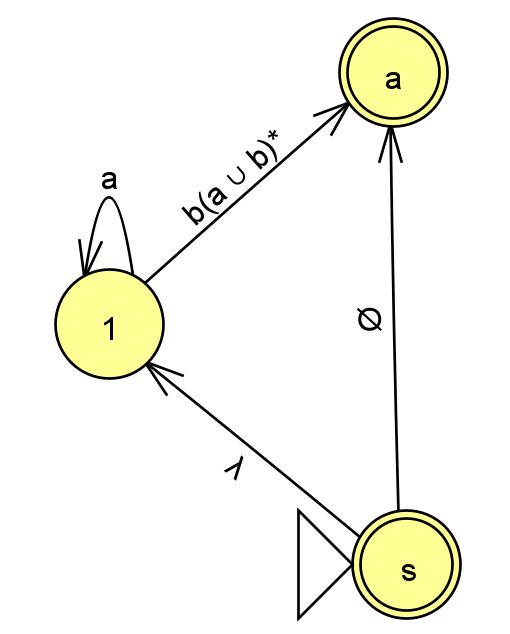
\includegraphics[scale=0.4]{assets/dfa_regex_3.png}
    \end{center}

    \item We do this process again. We pick our one non-start/accept state as $q_{\text{rip}} = 1$. By our algorithm again, let $q_i = s$ and $q_j = a$. Then: 
    \begin{itemize}
        \item $\delta(q_i, q_{\text{rip}}) = R_1 = \epsilon$
        \item $\delta(q_{\text{rip}}, q_{\text{rip}}) = R_2 = a$
        \item $\delta(q_{\text{rip}}, q_j) = R_3 = b(a \cup b)^*$
        \item $\delta(q_i, q_j) = R_4 = \emptyset$
    \end{itemize}
    Therefore, $\delta'(q_i, q_j) = (\epsilon)(a)^* b(a \cup b)^* \cup \emptyset$. This can be simplified to $\delta'(q_i, q_j) = (a)^* b(a \cup b)^*$. So, the corresponding new state diagram is:
    \begin{center}
        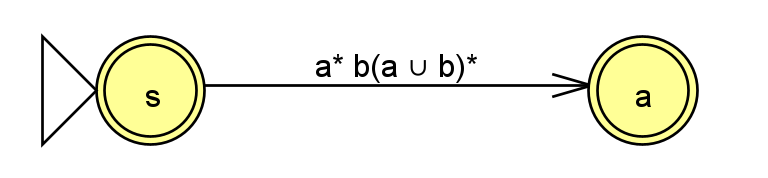
\includegraphics[scale=0.4]{assets/dfa_regex_4.png}
    \end{center}
    Thus, the regular expression corresponding to the given DFA is $\boxed{(a)^* b(a \cup b)^*}$
\end{enumerate}

% Ø  ∪ λ


\subsection{Regular Expressions and Regularity of Language}
\begin{theorem}{}{}
    A language is regular if and only if some regular expression describes it. 
\end{theorem}

\begin{mdframed}[]
    \begin{proof}
        The proof is given by the two lemmas. 
    \end{proof}    
\end{mdframed}

\subsubsection{Regular Expression Implies Regularity}

\begin{lemma}{}{}
    If a language is described by a regular expression, then it is regular. 
\end{lemma}

\begin{mdframed}[]
    \begin{proof}
        Suppose we convert $R$ into an NFA $N$. We then need to consider six cases as defined by the formal definition of regular expression.
        \begin{enumerate}
            \item Let $R = a$ for some $a \in \Sigma$. Then, $L(R) = \{a\}$ and the following NFA recognizes $L(R)$:
            \begin{center}
                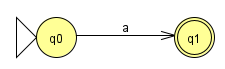
\includegraphics[scale=0.75]{assets/nfa_regex_pf_1.png}
            \end{center}
            
            \item Let $R = \epsilon$. Then, $L(R) = \{\epsilon\}$ and the following NFA recognizes $L(R)$:
            \begin{center}
                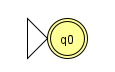
\includegraphics[scale=0.75]{assets/nfa_regex_pf_2.png}
            \end{center}

            \item Let $R = \emptyset$. Then, $L(R) = \emptyset$ and the following NFA recognizes $L(R)$:
            \begin{center}
                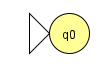
\includegraphics[scale=0.75]{assets/nfa_regex_pf_3.png}
            \end{center}

            \item $R = R_1 \cup R_2$
            \item $R = R_1 \circ R_2$
            \item $R = R_{1}^*$
        \end{enumerate}
        Where the last three cases is given by a previous proof. 
    \end{proof}
\end{mdframed}

\subsubsection{Regularity Implies Regular Expression}

\begin{lemma}{}{}
    If a language is regular, then it is described by some regular expression.
\end{lemma}

\begin{mdframed}[]
    \begin{proof}
        If the language is regular, then it is accepted by a DFA. From the above, we've given a sketch of how to convert a DFA to a regular expression. 
    \end{proof}
\end{mdframed}















\newpage 
\section{Nonregular Languages (1.4)}
Of course, with great power comes great responsibility. This is certainly the case with finite automata. That is, we will prove that certain languages cannot be recognized by any finite automaton. Consider the language
\[B = \{\code{0}^n \code{1}^n \mid n \geq 0\}\]
It's not possible for us to find a finite automaton that recognizes $B$ simply because the machine needs to remember how many \code{0}s have been seen so far as it reads the input. In other words, because the number of \code{0}s is not limited, the machine would have to keep track of an \emph{unlimited} number of possibilities.

\begin{note}{}{}
    Just because the language appears to require unbounded memory doesn't mean that it is necessarily non-regular. For example, consider the two languages over $\Sigma = \{\code{0}, \code{1}\}$: 
    \[C = \{w \mid w \text{ has an equal number of \code{0}s and \code{1}s}\}\]
    \[D = \{w \mid w \text{ has an equal number of occurrences of \code{01} and \code{10} as substrings}\}\]
    $C$ is not regular, but $D$ \emph{is} regular, despise the fact that both languages require a machine that might need to keep count. 
\end{note}

\subsection{The Pumping Lemma}
We can use the concept known as the pumping lemma to prove nonregularity. In particular, this theorem states that all regular languages have a special property: the property that all strings in the language can be \emph{pumped} if they are at least as long as a certain special value, called the \textbf{pumping length}. This means that each string contains a section that can be repeated \emph{any number of times} with the resulting string remaining in the language. 

\bigskip 

So, if we can show that a language doesn't have this property, then it must be true that this language isn't regular. 

\begin{theorem}{Pumping Lemma}{}
    If $A$ is a regular language, then there is a number $p$ (the \emph{pumping length}) where if $s$ is any string in $A$ of length at least $p$, then $s$ may be divided into three pieces, $s = xyz$, satisfying the following conditions: 
    \begin{enumerate}
        \item For each $i \geq 0$, $xy^i z \in A$
        \item $|y| > 0$
        \item $|xy| \leq p$
    \end{enumerate}
\end{theorem}
\textbf{General Remarks:}
\begin{itemize}
    \item The pumping lemma is used to prove that a language is not regular. It cannot be used to prove that a language is regular. 
\end{itemize}
\textbf{Notational Remarks:}
\begin{itemize}
    \item Recall that $|s|$ represents the length of a string $s$.
    \item $y^i$ means that $i$ copies of $y$ are concatenated together. 
    \item $y^0 = \epsilon$.
    \item When $s$ is divided into $xyz$, either $x$ or $z$ may be $\epsilon$, but $y \neq \epsilon$ by condition 2. 
\end{itemize}

\subsection{Using Pumping Lemma in Proofs}
To prove that a language $L$ is not regular, we use the pumping lemma like so: 
\begin{enumerate}
    \item Assume that $L$ is regular so that the Pumping Lemma holds.
    \item Let $p$ be the pumping length for $L$ given by the lemma.
    \item Find a string $s \in L$ such that $|s| \geq p$. Your $s$ must be parametrized by $p$. \textbf{Warning:} Not every string in $L$ will work. 
    \item By the Pumping Lemma, there are strings $x$, $y$, $z$ such that all three conditions hold. Pick a particular $i \geq 0$ (usually, $i = 0$ or $i = 2$ will suffice) and show that $xy^i z \notin L$, thus yielding a contradiction. 
\end{enumerate}
Several points to consider:
\begin{itemize}
    \item Your proof must show that, for an \underline{arbitrary} $p$, there is a \underline{particular} string $s \in L$ (long enough) such that for \underline{any} split of $xyz$ (satisfying the conditions), there is an $i$ such that $xy^i z \notin L$. In other words, you must: 
    \begin{itemize}
        \item Assume a general $p$. You \textbf{cannot} choose a particular $p$.
        \item Find a concrete $s$. Your $s$ must be parametrized by $p$.
        \item Consider a general split $x, y, z$. You \textbf{cannot} choose a particular split; you must show every possible split.
        \item Show a particular $i$ for which the pumped word is not in $L$.  
    \end{itemize}
    \item The string $s$ does not need to be a random, representative member of $L$. It may come from a \emph{very specific} subset of $L$. For example, if your language is all strings with an equal number of \code{0}'s and \code{1}'s, your $s$ might be $0^p 1^p$.
    \item Make sure your string is long enough so that the first $p$ characters have a very limited form. 
    \item The vast majority of proofs use $i = 0$ or $i = 2$, but there are exceptions. 
\end{itemize}

\subsubsection{Example 1: Pumping Lemma Application}
We will show that the language $B$ described above is not regular.

\begin{mdframed}[]
    \begin{proof}
        Assume to the contrary that $B$ is regular. Then, let $p$ be the pumping length given by the pumping lemma. Let $s$ be the string $\code{0}^p \code{1}^p$. Because $s \in B$ and $|s| = 2p > p$, the pumping lemma guarantees that $s$ can be split into three pieces, $s = xyz$, where for any $i \geq 0$ the string $xy^i z \in B$. We now consider three cases to show that this is impossible. 
        \begin{enumerate}
            \item The string $y$ consists of only \code{0}s. In this case, the string $xyyz$ has more \code{0}s than \code{1}s and so is not a member of $B$, violating condition 1 of the pumping lemma. 
            \item The string $y$ consists of only \code{1}s. This also violates condition 1 of the pumping lemma. 
            \item The string $y$ consists of both \code{0}s and \code{1}s. In this case, the string $xyyz$ may have the same number of \code{0s} and \code{1}s, but they will be out of order since some \code{1}s will come before \code{0}s.
        \end{enumerate}
        Hence, a contradiction is unavoidable if we make the assumption that $B$ is regular. Thus, $B$ cannot be regular. 
    \end{proof}
\end{mdframed}
\textbf{Remark:} If we applied condition 3 of the Pumping Lemma, we could have removed case 2 and 3. An alternative proof is given below. 
\begin{mdframed}[]
    \begin{proof}
        Assume to the contrary that $B$ is regular. Then, let $p$ be the pumping length given by the pumping lemma. Let $s$ be the string $\code{0}^p \code{1}^p$. Because $s \in B$ and $|s| = 2p > p$, the pumping lemma guarantees that $s$ can be split into three pieces, $s = xyz$, where for any $i \geq 0$ the string $xy^i z \in B$. If our string looks like: 
        \[s = \overbrace{0000 \dots 0000}^{p \text{ times}} \overbrace{1111 \dots 1111}^{p \text{ times}}\]
        Then, we can split the string like so: 
        \[s = \underbrace{000}_{x}\overbrace{0 \dots 0000}^{y} \underbrace{1111 \dots 1111}_{z}\]
        Suppose $x$ has length $a$ and $y$ has length $b$ where $a + b \leq p$. Then, for $i = 2$, we have the string $xyyz$ where $xyy$ has length $a + b + b > p$ while $z$ has length $p$, a contradiction since we must have the same length of \code{0} and \code{1}. 
    \end{proof}
\end{mdframed}



\end{document}